\chapter{System Design and Implementation}%
\label{chapter:systemDesignandImplementation}

\begin{introduction}
This chapter presents the design and implementation of the system. It begins with the database structure, organized into six core areas to support all workflows described in the previous chapter. Following this, the application views are detailed, illustrating how each user role — receptionist, mechanic, warehouse operator, workshop manager, client, and administrator — interacts with the system through tailored interfaces. The chapter concludes with a summary showing that the implemented views collectively fulfill the defined system requirements.
\end{introduction} 


\section{Database}


\subsection{Structure} 



The database was designed to support all the workflows described in the previous sections, ensuring that the system could track users, vehicles, maintenance tasks, parts, purchases, and dealership partnerships in a consistent way. The overall structure is shown in Figure~\ref{fig:dbGeneral}, which organizes the database into six main areas:
 
\begin{itemize}
  \item Users
  \item Maintenance and Tasks
  \item Parts and Inventory 
  \item Purchasing
  \item Services
  \item Vehicles and Owners
\end{itemize}

Tables that already existed in the original Lightmobie database are marked with a red dot in the diagrams.

\begin{figure}[h]
  \caption{Database general diagram.}
  \centering
  \includegraphics[width=0.75\textwidth]{figs/dbDiagrams/DbDiagramFull}
  \label{fig:dbGeneral} 
\end{figure}



\subsubsection{Users} 

The user section builds on the existing Lightmobie database. It manages user accounts, their roles (e.g., client, receptionist, mechanic, warehouse operator, administrator), and user groups. This structure defines the system’s access control and ensures that each type of user can only perform their intended operations.

Figure~\ref{fig:dbUsers} shows this structure.

\begin{figure}[h]
  \caption{Database diagram for Users.}
  \centering
  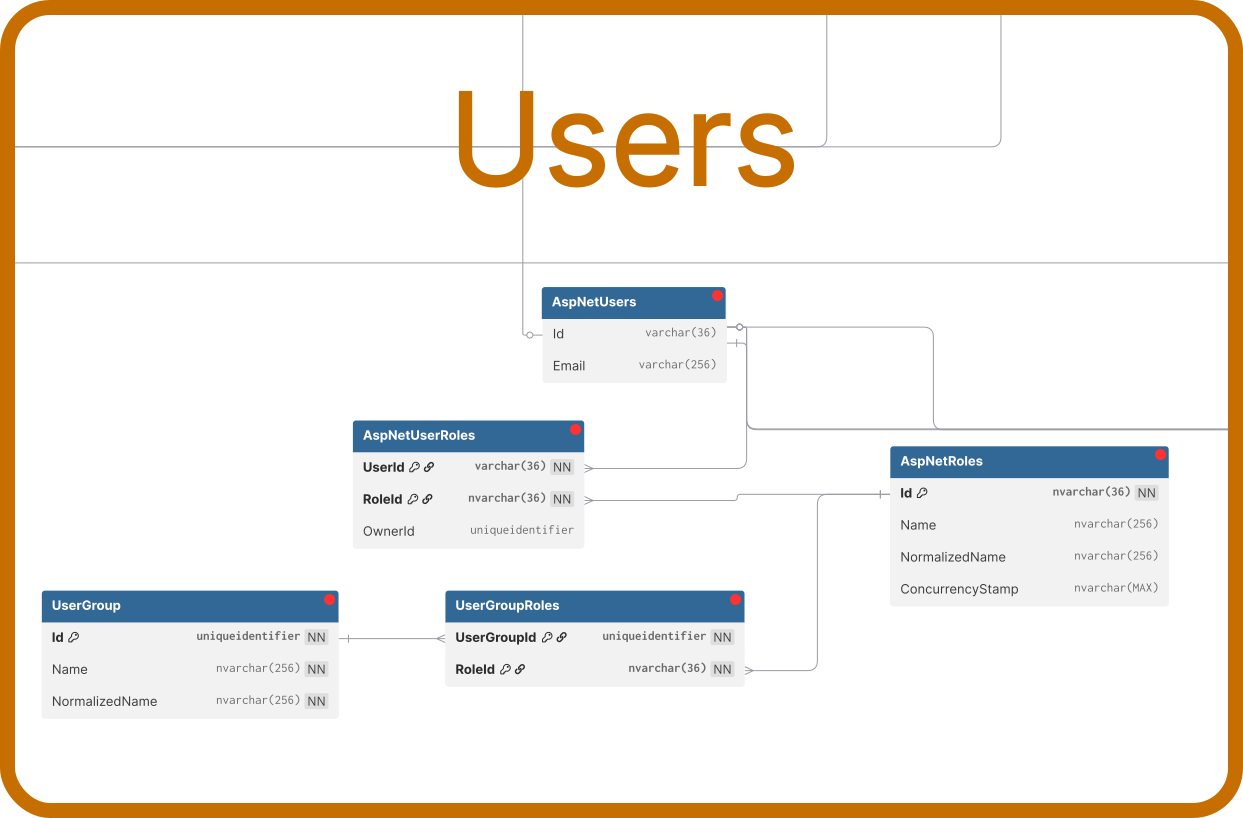
\includegraphics[width=0.75\textwidth]{figs/dbDiagrams/Users}
  \label{fig:dbUsers}
\end{figure}


\subsubsection{Maintenance and Tasks} 


Maintenance is at the core of the system. Each maintenance record links a client, a dealership, and a vehicle, and stores important information such as evaluation results, expected and actual budgets, delivery dates, and quality scores.

Tasks are associated with a maintenance and describe the specific operations to be performed. Each task can have a status (e.g., waiting for client approval, assigned to a mechanic, waiting for parts, concluded), can be paused, and is eventually completed by a mechanic.

The system also supports maintenance changes (e.g., delays, budget adjustments, or task cancellations). These are stored separately so that all modifications can be tracked and require explicit validation from the client.

Figure~\ref{fig:dbMaintenance} illustrates this structure.

\begin{figure}[h]
  \caption{Database diagram for Maintenance and Tasks.}
  \centering
  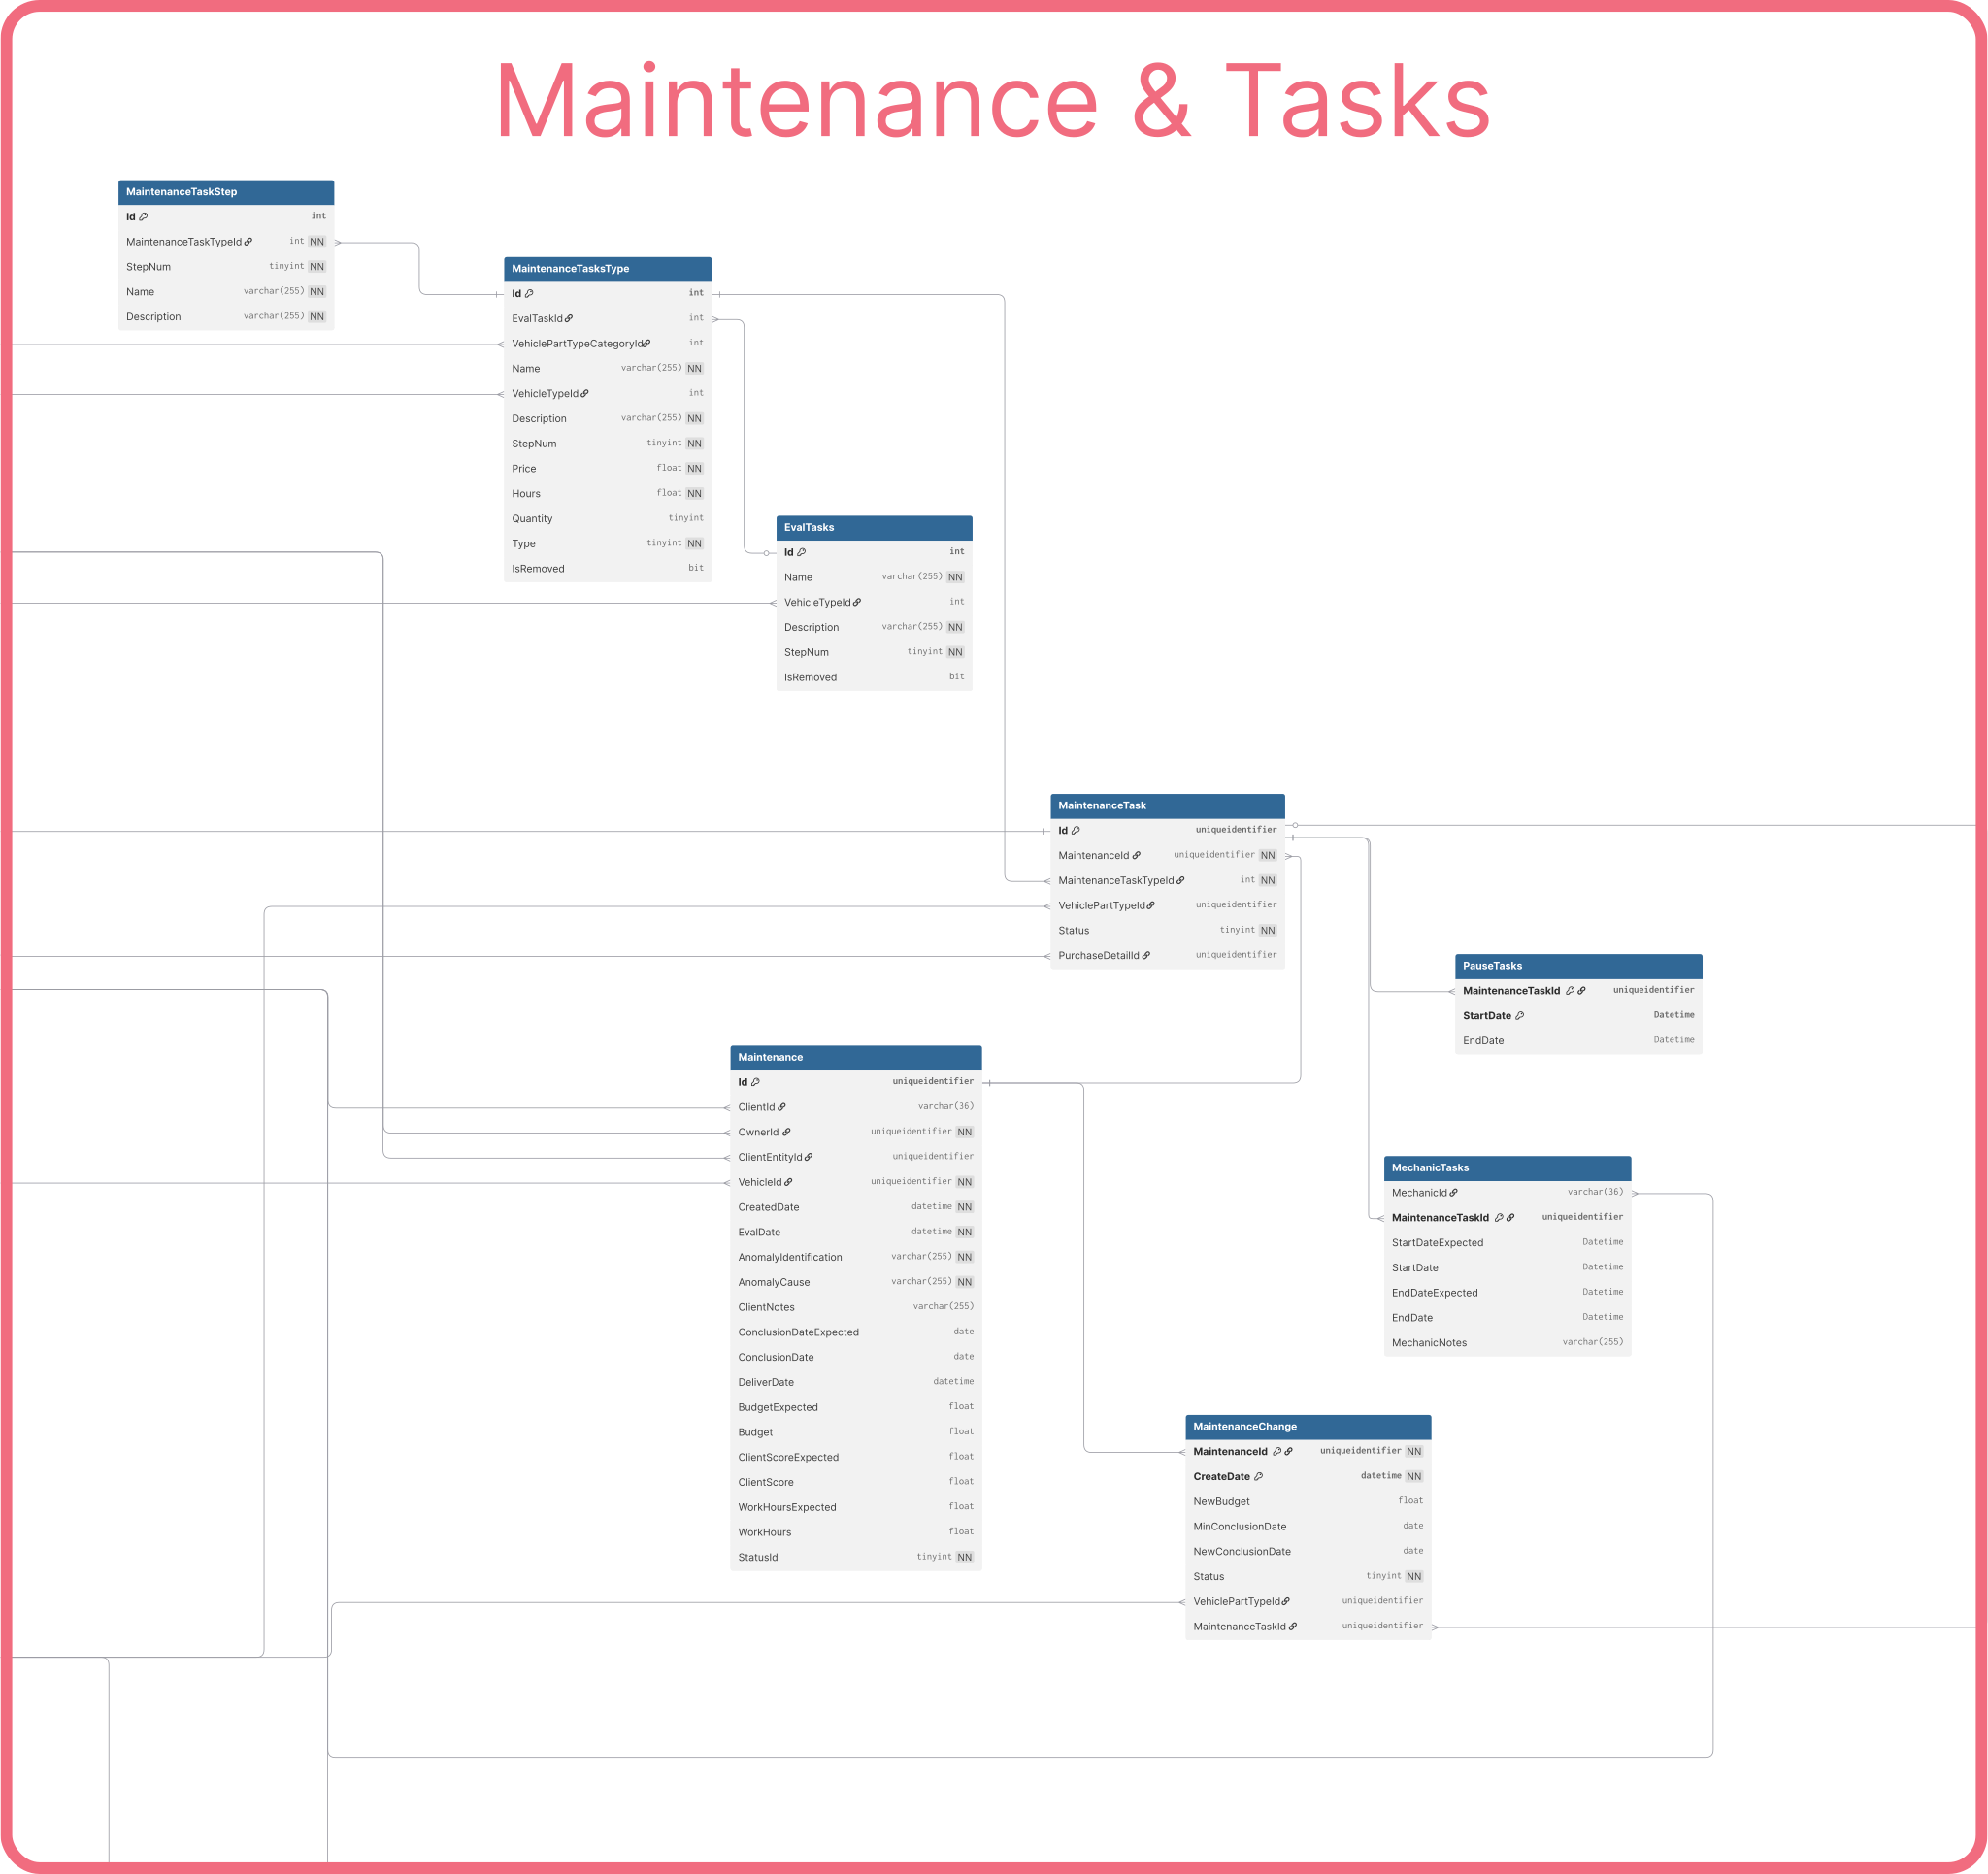
\includegraphics[width=0.75\textwidth]{figs/dbDiagrams/Maintenance_and_Tasks}
  \label{fig:dbMaintenance}
\end{figure}



\subsubsection{Parts and Inventory} 


The inventory section keeps track of all parts available at a dealership. For each part, the system stores quantities, warehouse location, and stock thresholds to automate restocking when levels fall below a minimum.

Every change in stock (sales to mechanics, restocks from purchases) is logged as a transaction, which ensures traceability. The database also models suppliers and their contracts with dealerships, so the system knows which supplier provides which parts.

Figure~\ref{fig:dbParts} shows this structure.

\begin{figure}[h]
  \caption{Database diagram for Parts and Inventory.}
  \centering
  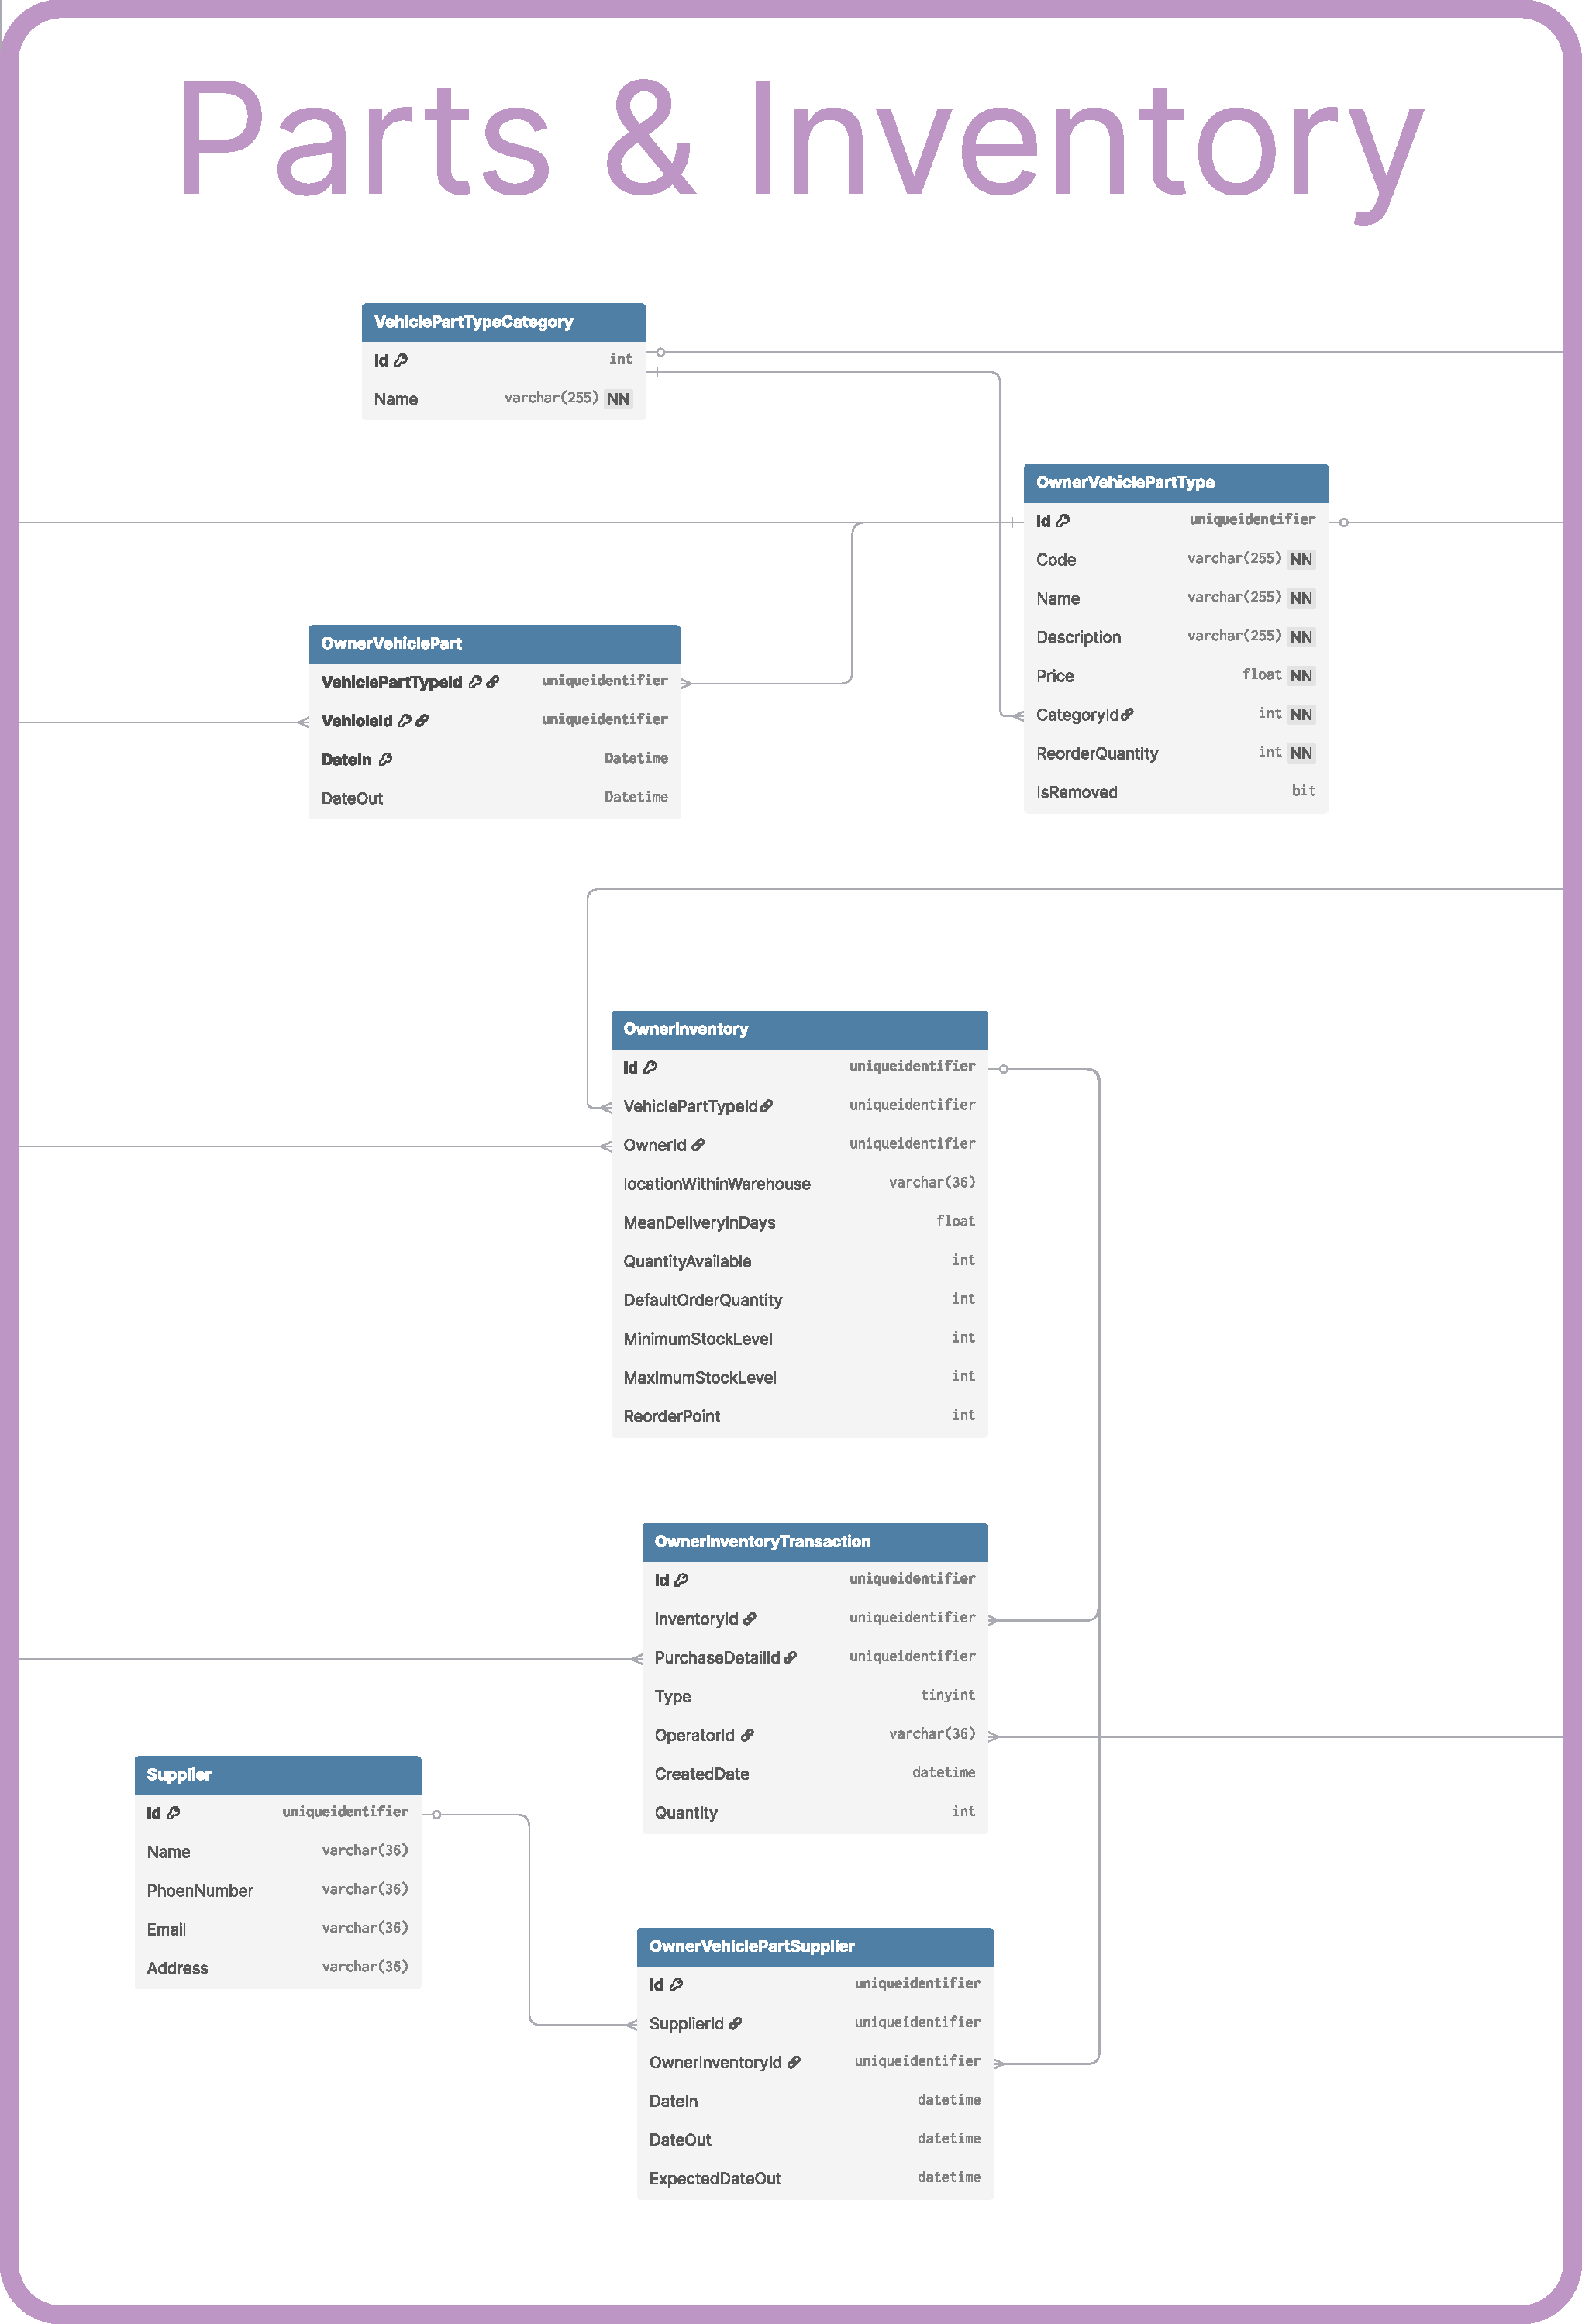
\includegraphics[width=0.75\textwidth]{figs/dbDiagrams/Parts_and_Inventory}
  \label{fig:dbParts}
\end{figure}


\subsubsection{Purchasing} 


When stock runs out, the system generates purchase requests. Each purchase goes through a workflow: waiting for approval by the workshop manager, assignment to a warehouse operator, ordering from a supplier, waiting for delivery, and finally being marked as finished once the parts arrive.

Purchase records store details of the items ordered, expected and actual arrival dates, and possible delays. Purchases can also be linked directly to maintenance tasks, ensuring that when parts arrive, the related tasks are updated automatically.

Figure~\ref{fig:dbPurchasing} illustrates the purchasing tables.

\begin{figure}[h]
  \caption{Database diagram for Purchasing.}
  \centering
  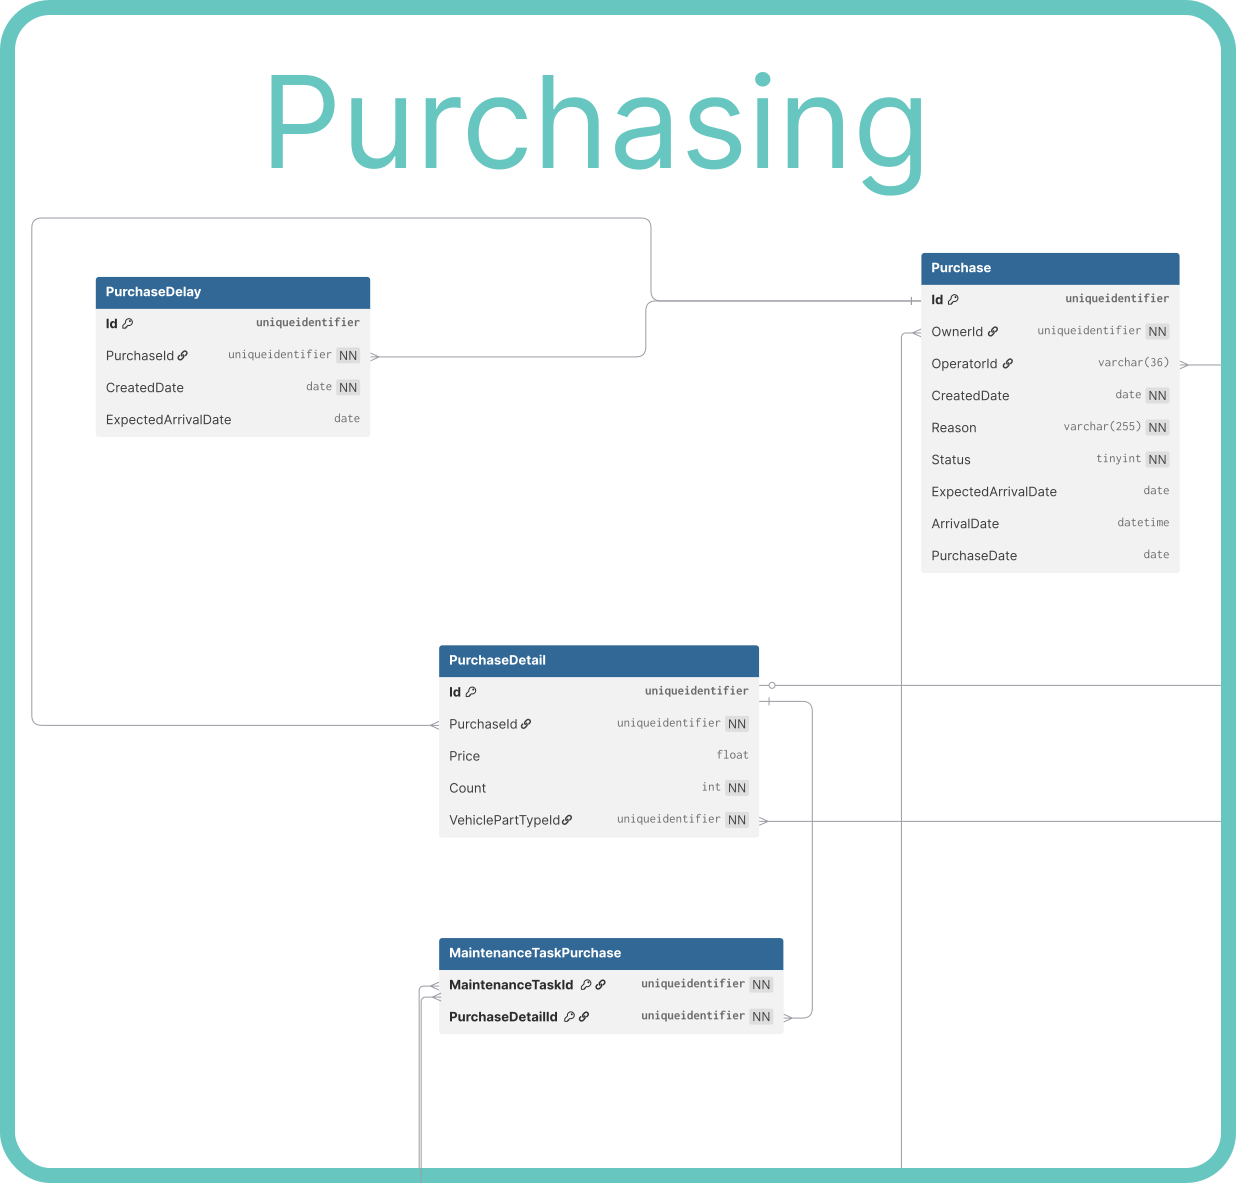
\includegraphics[width=0.75\textwidth]{figs/dbDiagrams/Purchasing}
  \label{fig:dbPurchasing}
\end{figure}


\subsubsection{Services} 

The services section defines the types of services supported by the system, such as dealership maintenance or bike-sharing fleet management. Since not all dealerships operate in the same way, this part of the database allows them to configure how their workflow should behave.

By storing these configuration options, the system adapts to different service models while maintaining a consistent data structure.

Figure~\ref{fig:dbServices} shows the services structure.

\begin{figure}[h]
  \caption{Database diagram for Services.}
  \centering
  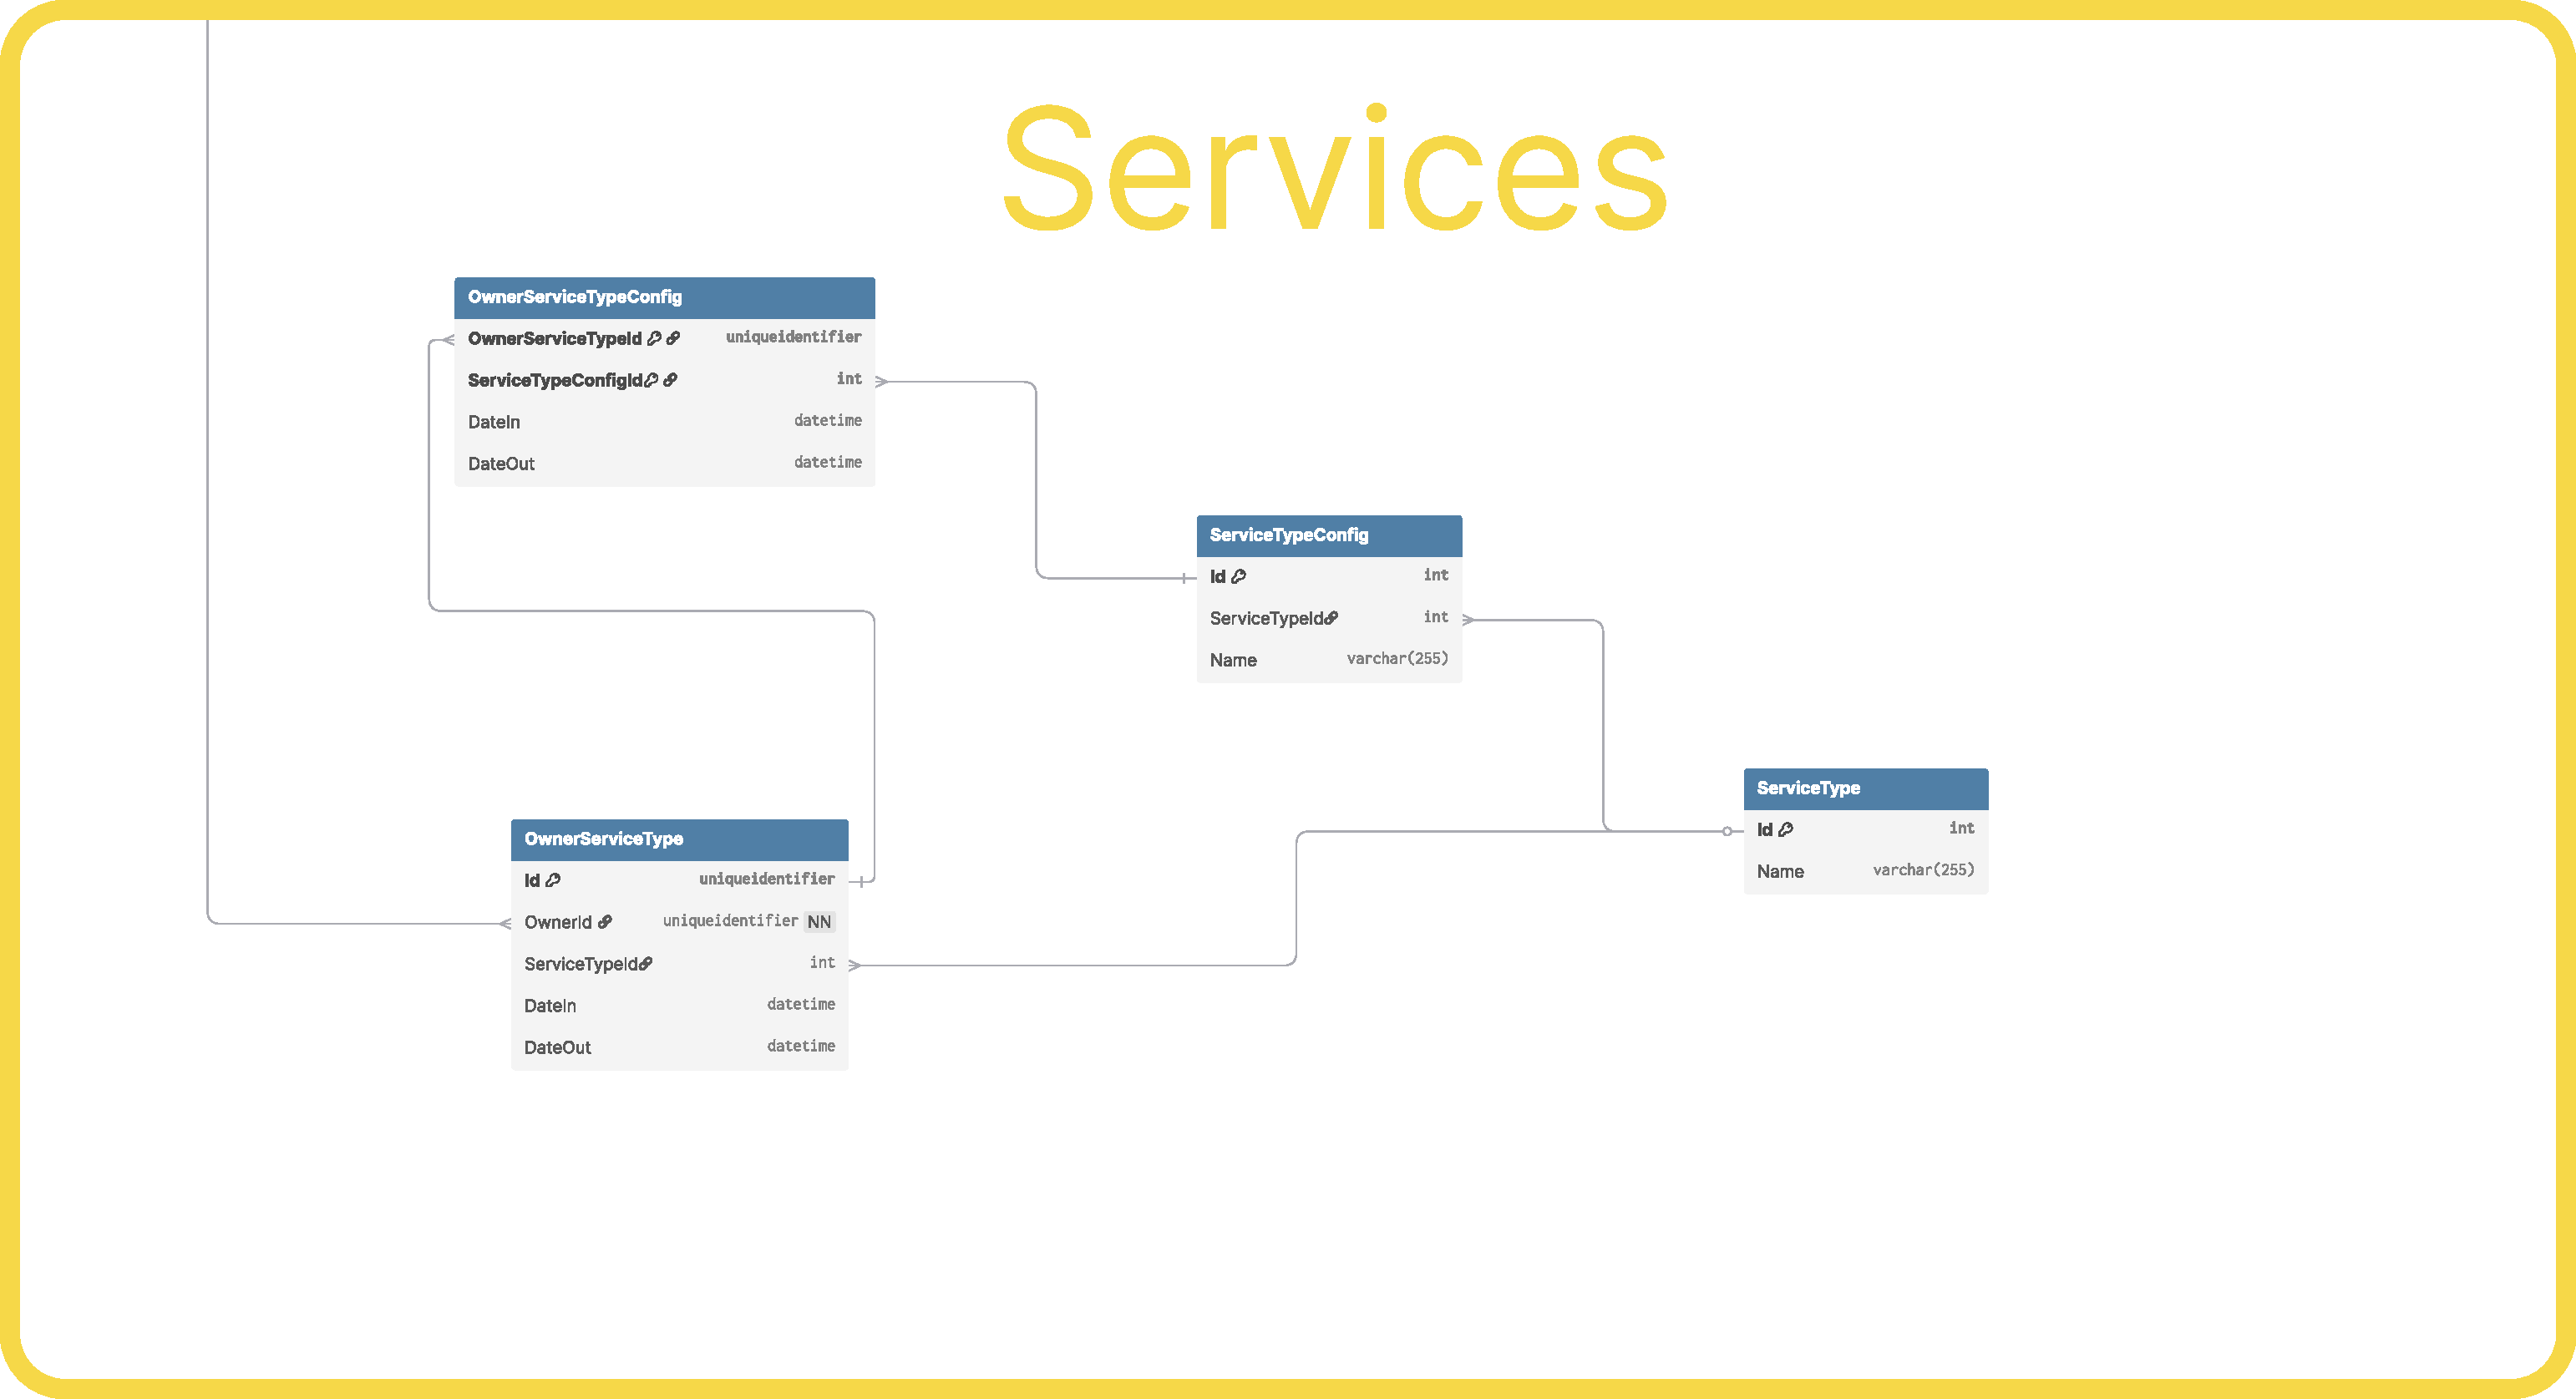
\includegraphics[width=0.75\textwidth]{figs/dbDiagrams/Services}
  \label{fig:dbServices}
\end{figure}


\subsubsection{Vehicles and Owners} 


Finally, the system manages dealerships, bike-sharing companies, and vehicles. Vehicles are linked to their type (e.g., electric bike, conventional bike) and to the dealership or entity that owns them.

Partnerships between bike-sharing companies and dealerships are also modeled, allowing bike-sharing entities to grant specific dealerships access to their fleet information. Each partnership request can be accepted, denied, or remain pending.

Figure~\ref{fig:dbVehicles} shows this part of the database.

\begin{figure}[h]
  \caption{Database diagram for Vehicles and Owners}
  \centering
  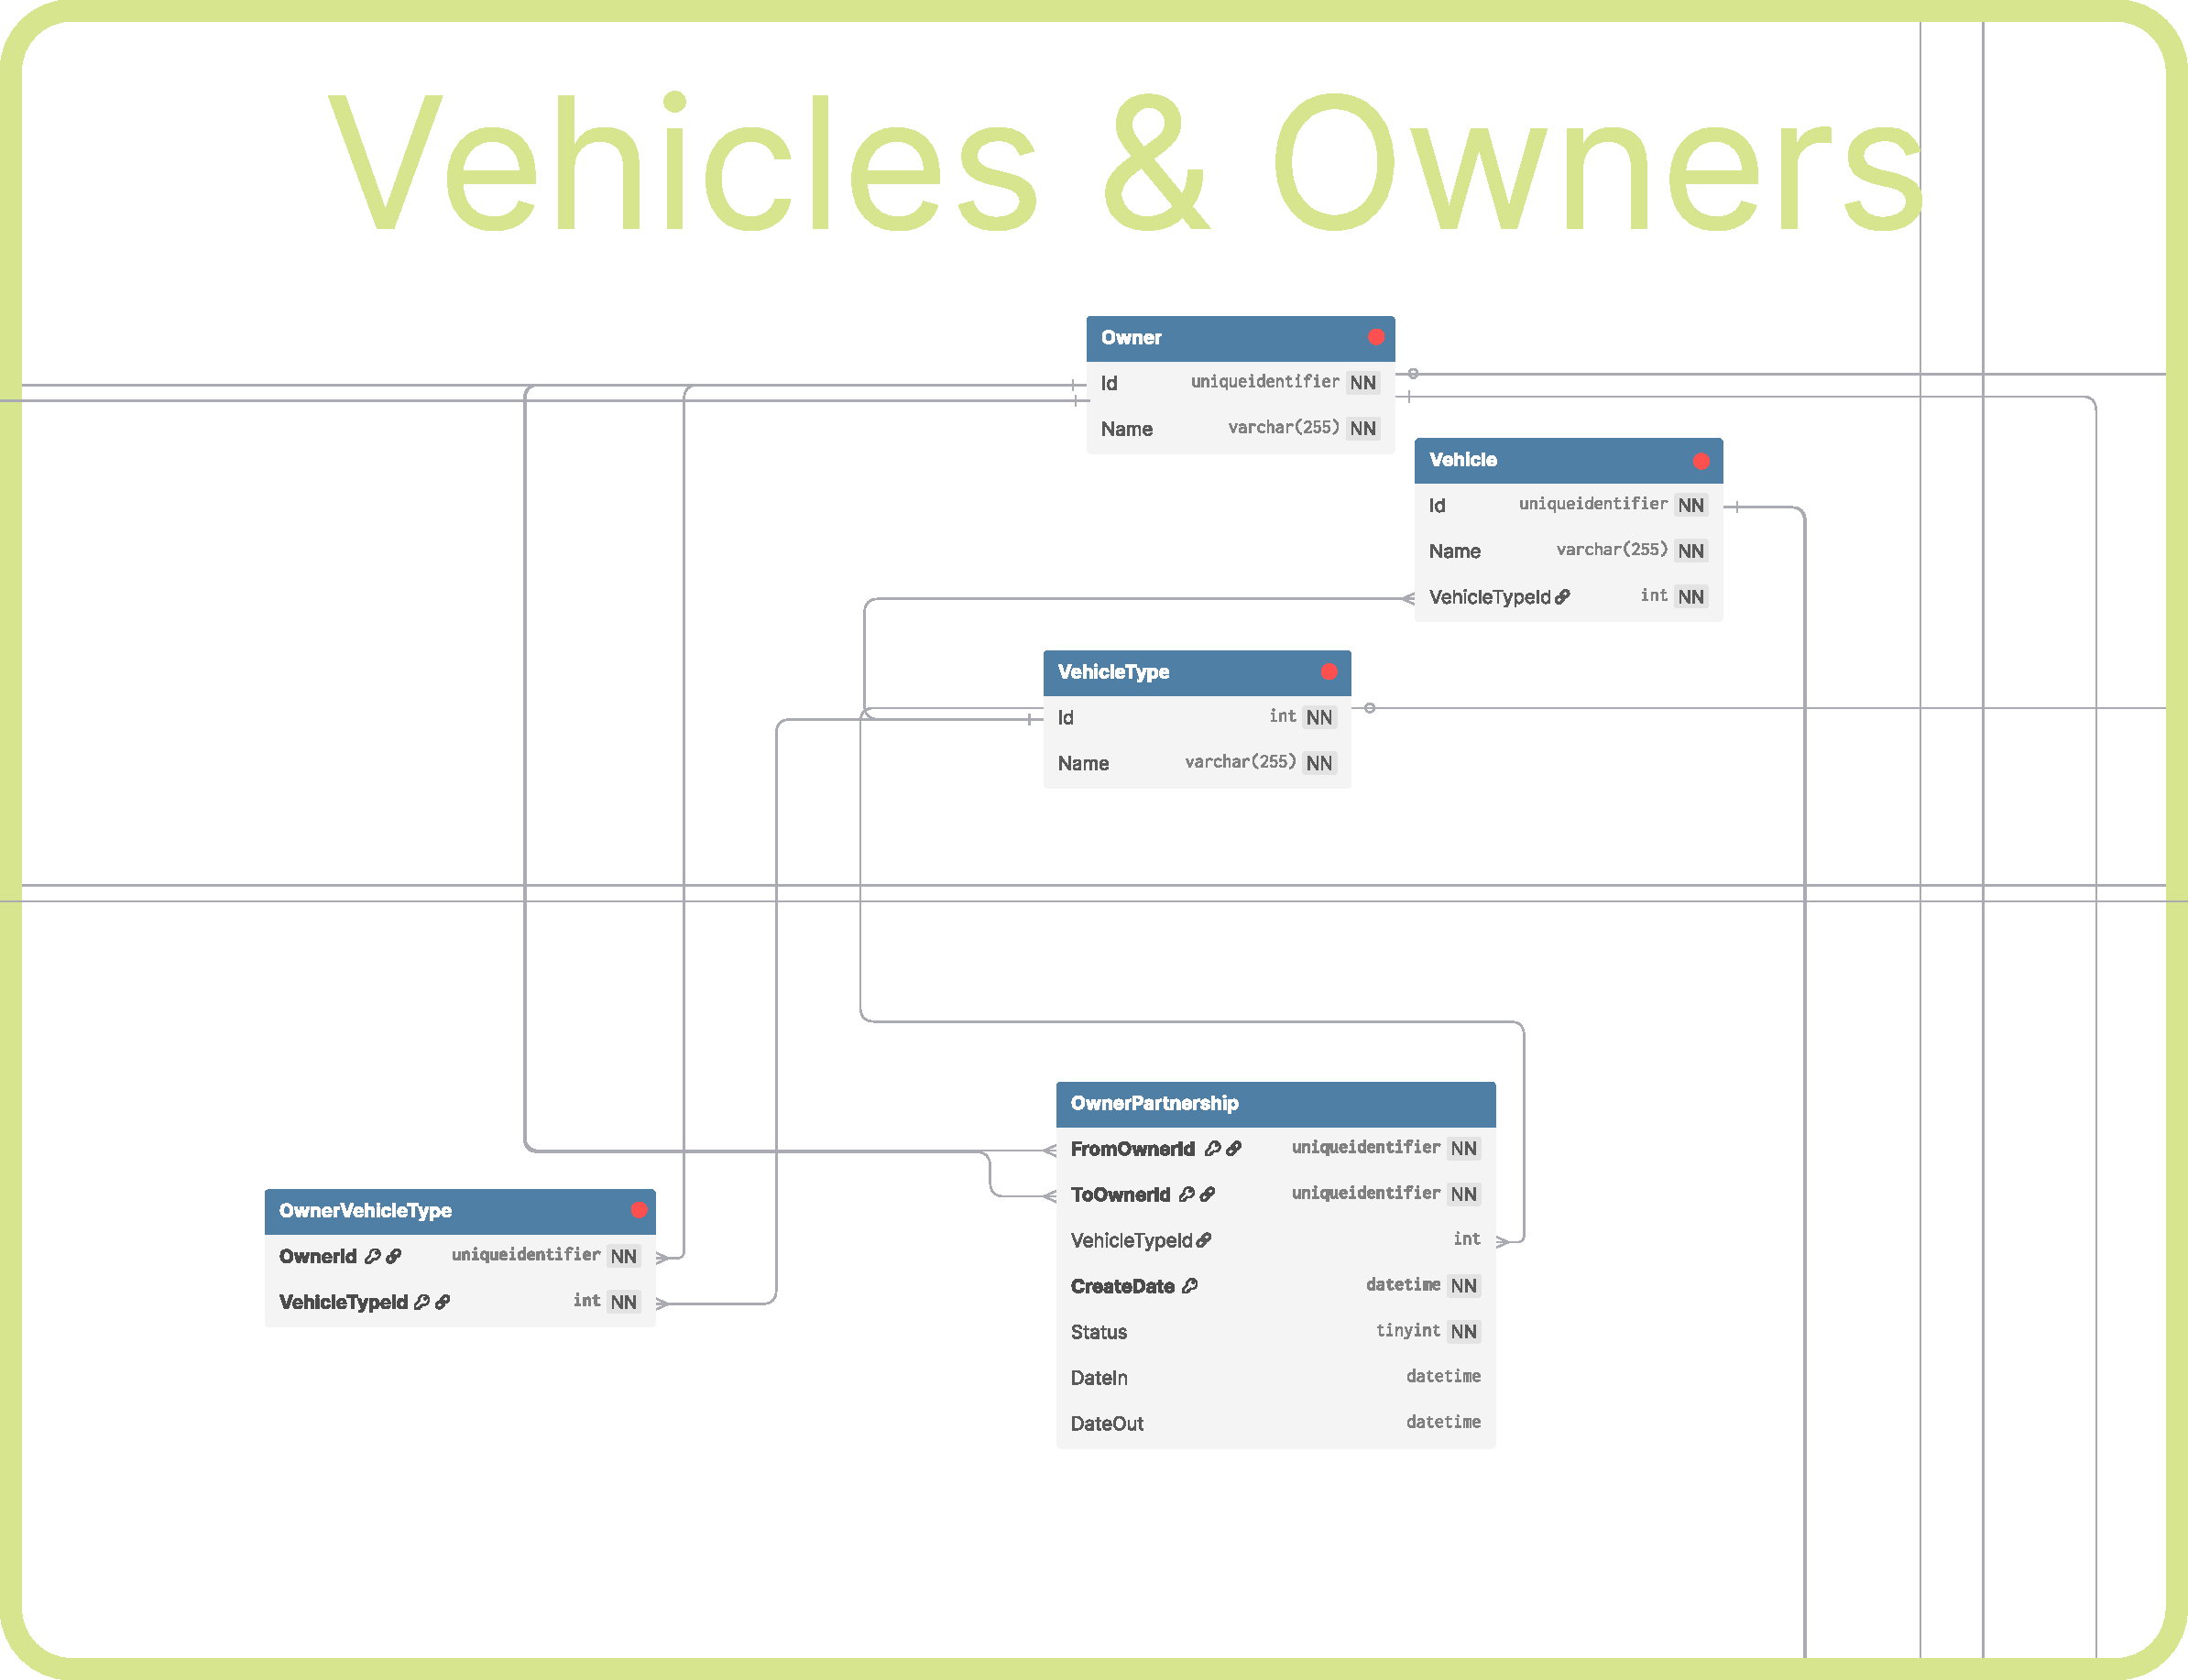
\includegraphics[width=0.75\textwidth]{figs/dbDiagrams/Vehicles_and_Owners}
  \label{fig:dbVehicles}
\end{figure}


Together, these six areas form an integrated database that supports the entire maintenance workflow. User accounts and roles define who can perform which actions, while vehicles and owners provide the foundation for creating maintenance records. Each maintenance can then be broken into tasks, which may require parts from inventory or trigger purchase requests. Services configure how dealerships organize these operations, ensuring flexibility across different business models. By connecting all these elements, the database ensures that every interaction—from a client request to the arrival of new parts—remains consistent, traceable, and adaptable to the needs of each dealership.

\subsection{Indexes and Stored Procedures}

To ensure the efficiency and consistency of the database, indexes and stored procedures were created to support the main operations of the system.

Indexes were added to optimize the execution of queries used most frequently. As indexes for primary keys are automatically created by the database, additional indexes were defined for all foreign keys and for the main filtering and sorting queries used in the application. These queries can be found in Figure~\ref{fig:BD_indexes-1}-\ref{fig:BD_indexes-4}.  

Stored procedures were also implemented to guarantee that operations involving multiple tables are executed atomically and consistently. These procedures handle actions that impact several parts of the system and must be completed as a single, coherent transaction. Examples include:

\begin{itemize}
  \item \textbf{Completing a mechanic's task}, since it affects the task, inventory, transaction, and vehicle parts tables, and may also update the maintenance if all tasks are concluded.
  \item \textbf{Assigning a task}, which modifies the \textit{maintenanceTask} and \textit{mechanicTasks} tables simultaneously.
  \item \textbf{Cancelling a maintenance}, which invalidates all pending tasks, updates the maintenance status, and discards pending maintenance changes.
  \item \textbf{Registering new parts}, which updates the purchase status, modifies the dealership's inventory, creates related transaction records, and updates maintenance tasks associated with the purchase.
\end{itemize}

These stored procedures ensure that the database maintains integrity and consistency during complex operations, reducing the risk of data conflicts and improving the reliability of the system.




\section{Implementation}

\subsection{Rececionist view}



\begin{figure}[h]
  \caption{Rececionist home page.}
  \centering
  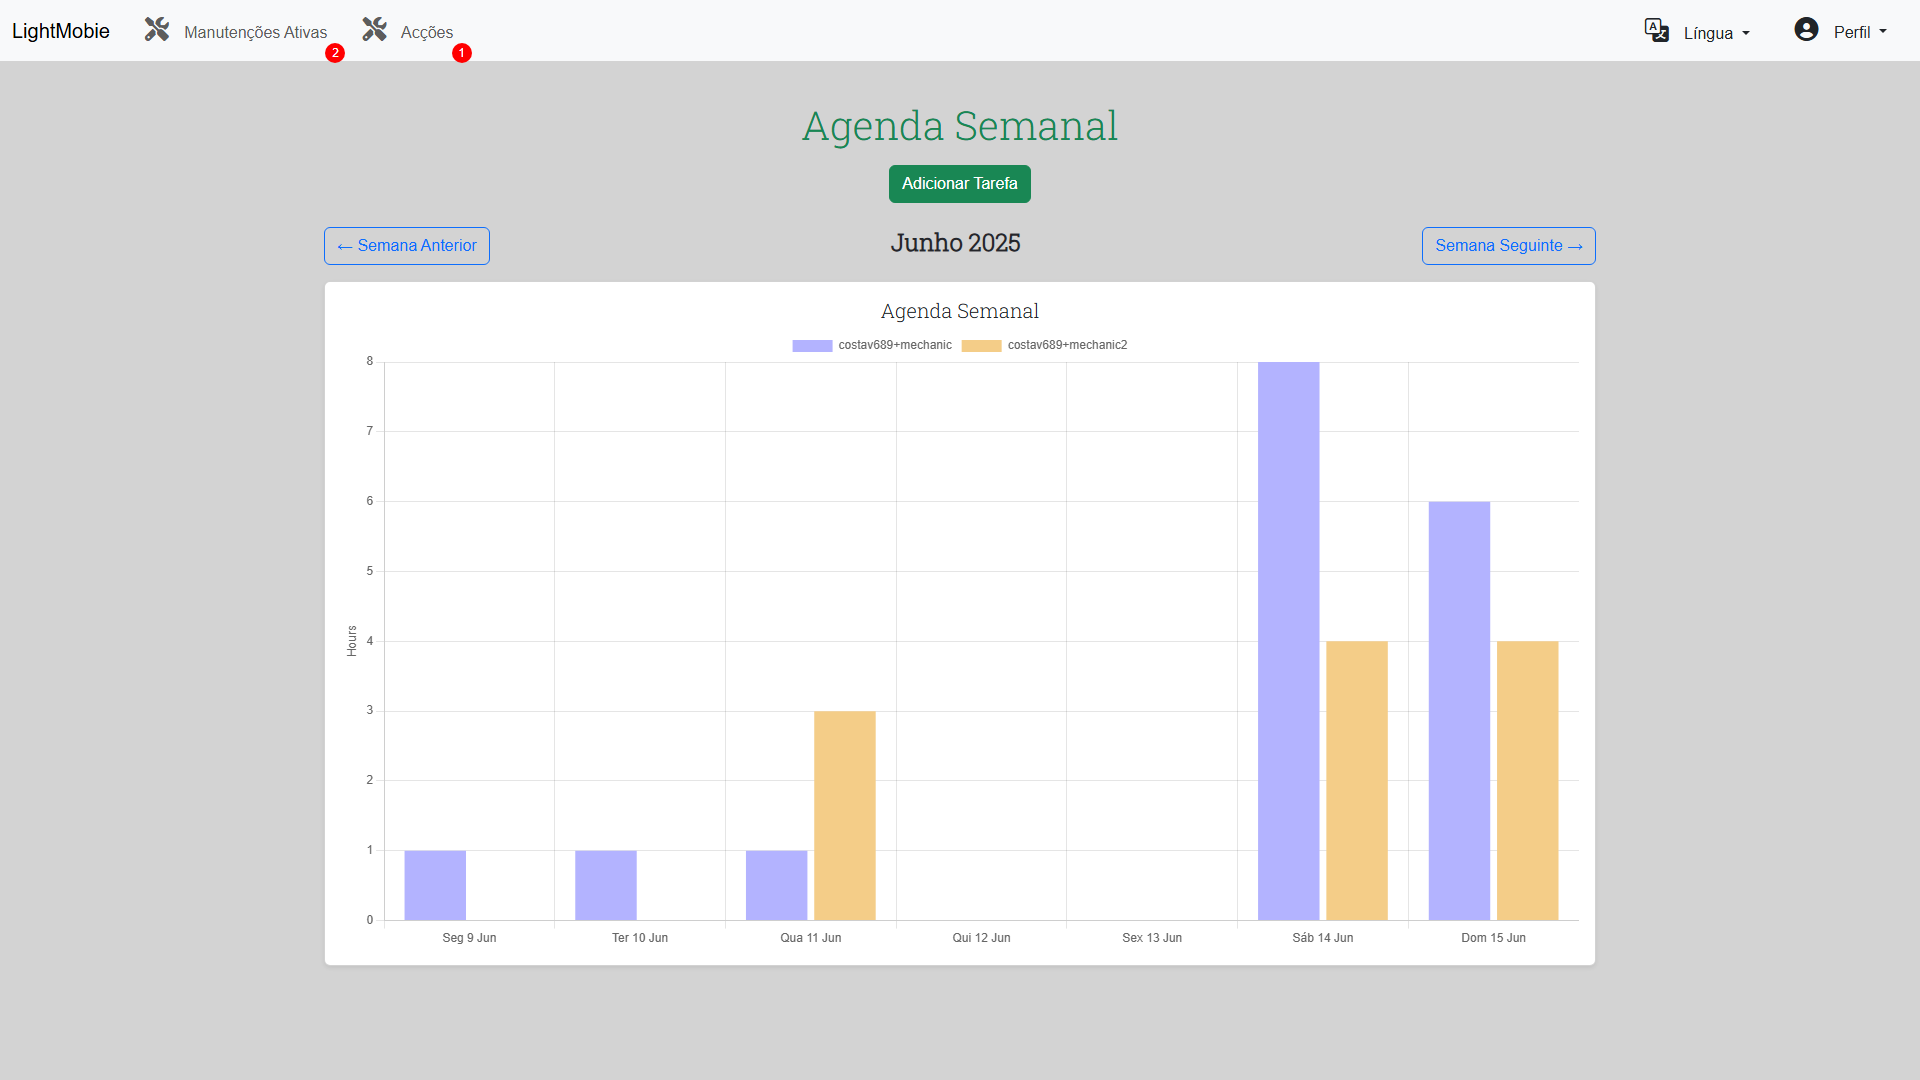
\includegraphics[width=\textwidth]{figs/Implementation/rececionist/rececionistHomePage}
  \label{fig:impReceHome}
\end{figure}

The receptionist's interface is designed to simplify the scheduling and monitoring of maintenance operations. Its main screen (Figure~\ref{fig:impReceHome}) presents a bar chart that displays the expected working hours of each mechanic for the selected week. Navigation buttons allow the receptionist to move between weeks, making it easy to identify which mechanics are available to perform vehicle evaluations. 


\begin{figure}[h]
  \caption{Rececionist schedule maintenance.}
  \centering
  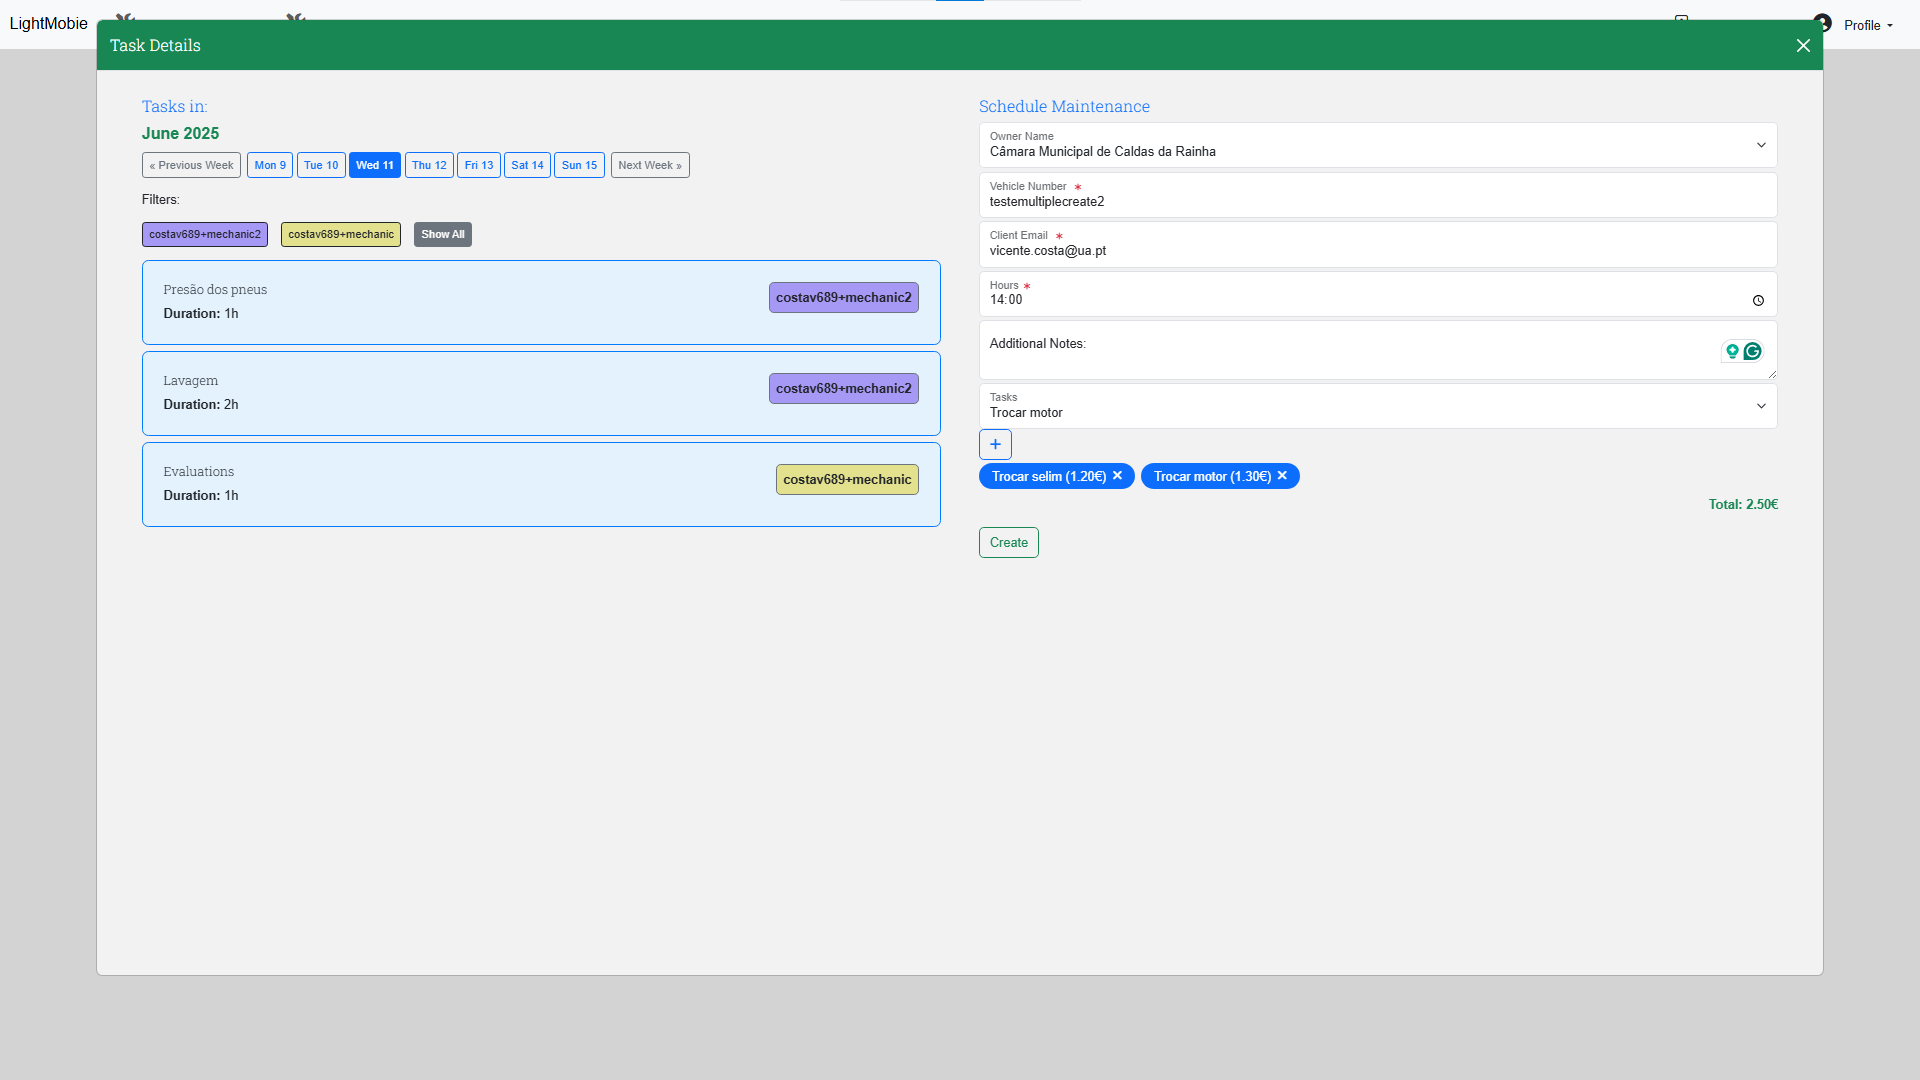
\includegraphics[width=\textwidth]{figs/Implementation/rececionist/addTask}
  \label{fig:impReceAddTask}
\end{figure}

To schedule a new maintenance, the receptionist can either click the "Schedule Maintenance" button or select a specific date on the chart. Both options open a modal (Figure~\ref{fig:impReceAddTask}), where the date can be adjusted, existing tasks for that day are displayed, and a scheduling form is available. The form includes fields for the client's information, vehicle registration, arrival time, optional pre-selected tasks, and notes for the mechanic. Once completed, the receptionist confirms the schedule, creating a new maintenance record in the system (Use Case 1.1 – Maintenance Schedule). If the email entered for the maintenance isn't linked to any existing client, the system automatically creates a new client record with just an ID and the email address. Then, an email is sent to the client with a link to a form where they can confirm their email, set a password, and fill in the rest of their information (Figures~\ref{fig:CreateClient} and ~\ref{fig:SetPassword}).

\begin{figure}[h]
  \caption{List of active maintenances.}
  \centering
  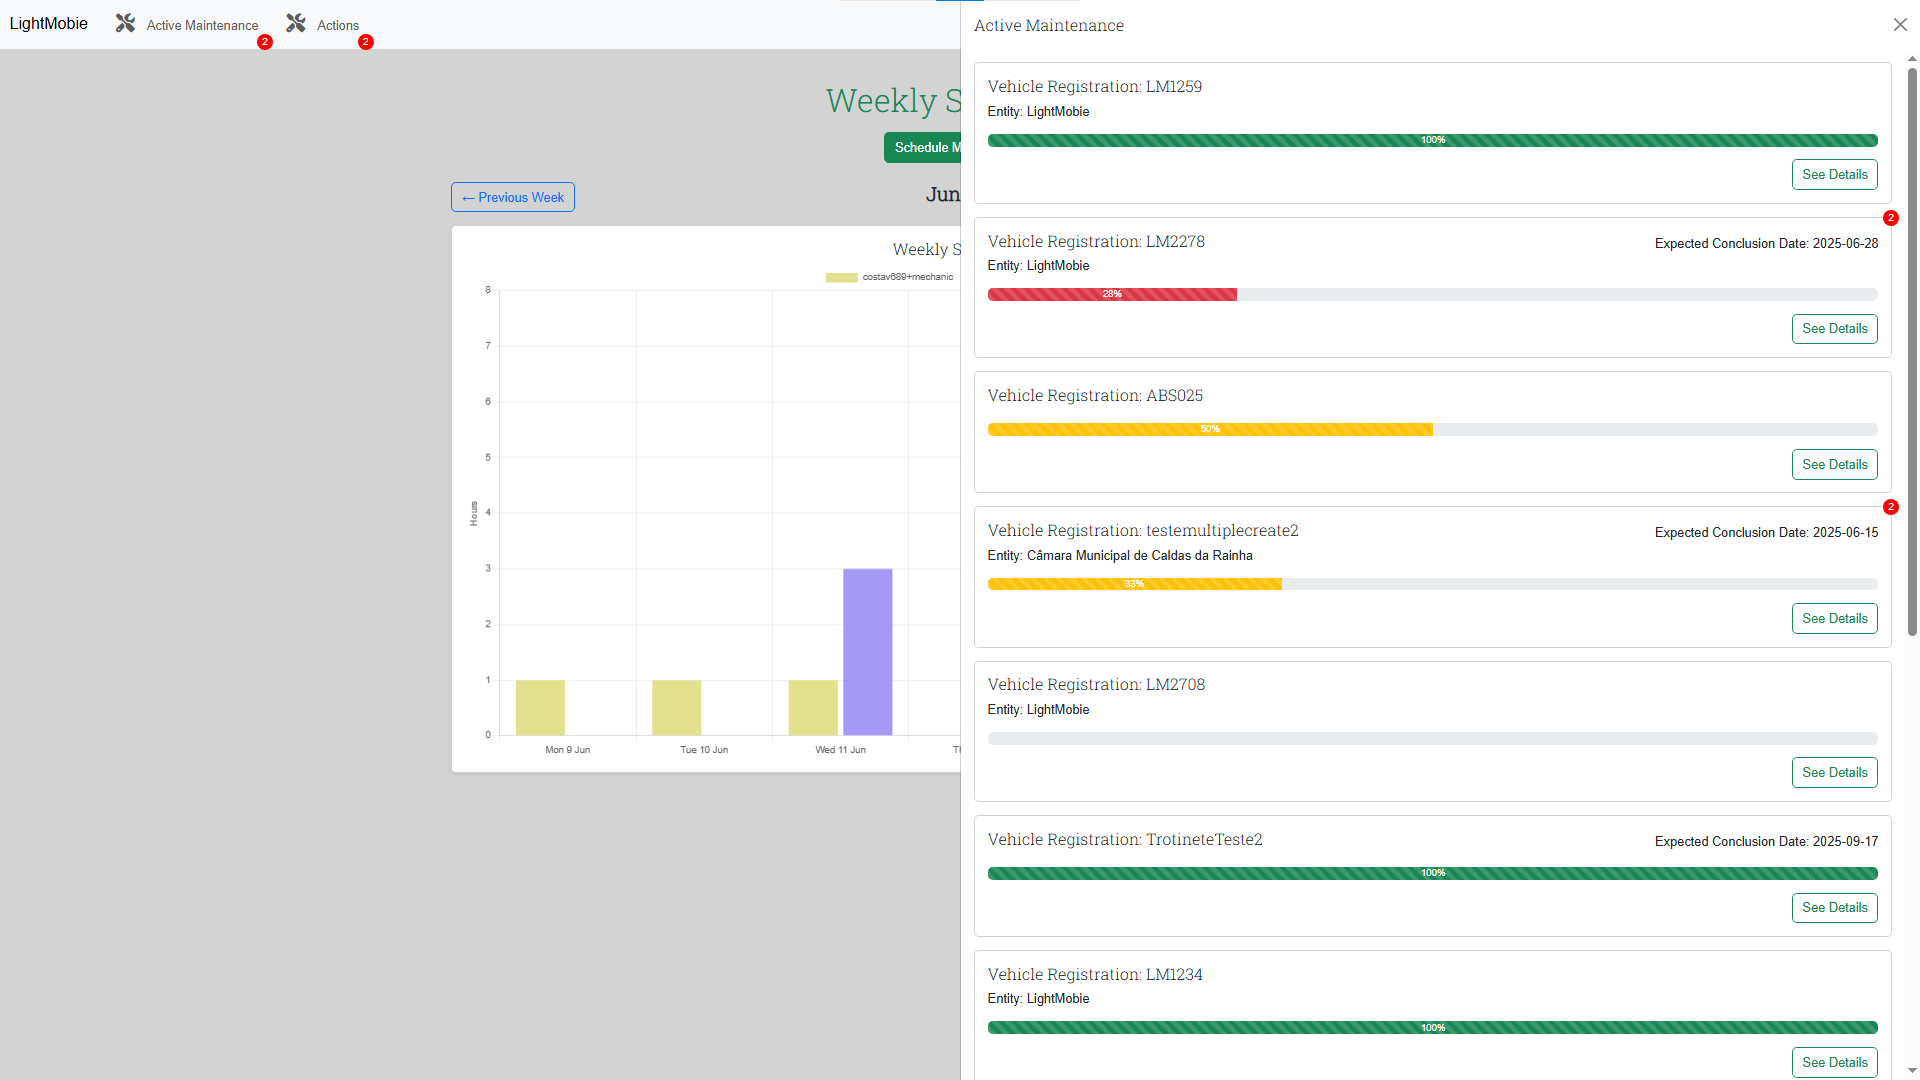
\includegraphics[width=\textwidth]{figs/Implementation/rececionist/activeMaintenances}
  \label{fig:impReceListMaint}
\end{figure}


The application also provides quick access to active maintenances through the "Active Maintenance" menu option (Figure~\ref{fig:impReceListMaint}). This section lists ongoing maintenances, including key details such as vehicle registration, associated entity, expected completion date, and progress percentage. Visual indicators highlight maintenances with pending changes requiring client confirmation. From here, the receptionist can open detailed views (Figures~\ref{fig:impReceMaintHome}, ~\ref{fig:impReceMaintTask} and ~\ref{fig:impReceMaintChange}), which present information about the maintenance, associated tasks, and any proposed changes. 
In addition, the modal includes a dedicated tab for the approval of maintenance tasks following the vehicle evaluation (Figure~\ref{fig:impReceMaintApproval}). In this tab, the receptionist can review the tasks proposed by the mechanic, their associated costs, required parts, and warehouse availability. Once the client's preferences are confirmed, the receptionist finalizes the maintenance plan (Use Case 1.2 – Define maintenance details).
These features enable the receptionist to respond accurately to client inquiries (Use Case 1.3 – Collect maintenance information) and manage approvals or cancellations of changes (Use Cases 1.4, 1.5, and 1.7). Additionally, the receptionist can complete the maintenace process by recording the vehicle delivery date (Use Case 1.6 – Deliver vehicle).



\begin{figure}[htbp]
  \caption{Active maintenance details approval tab.}
  \centering
  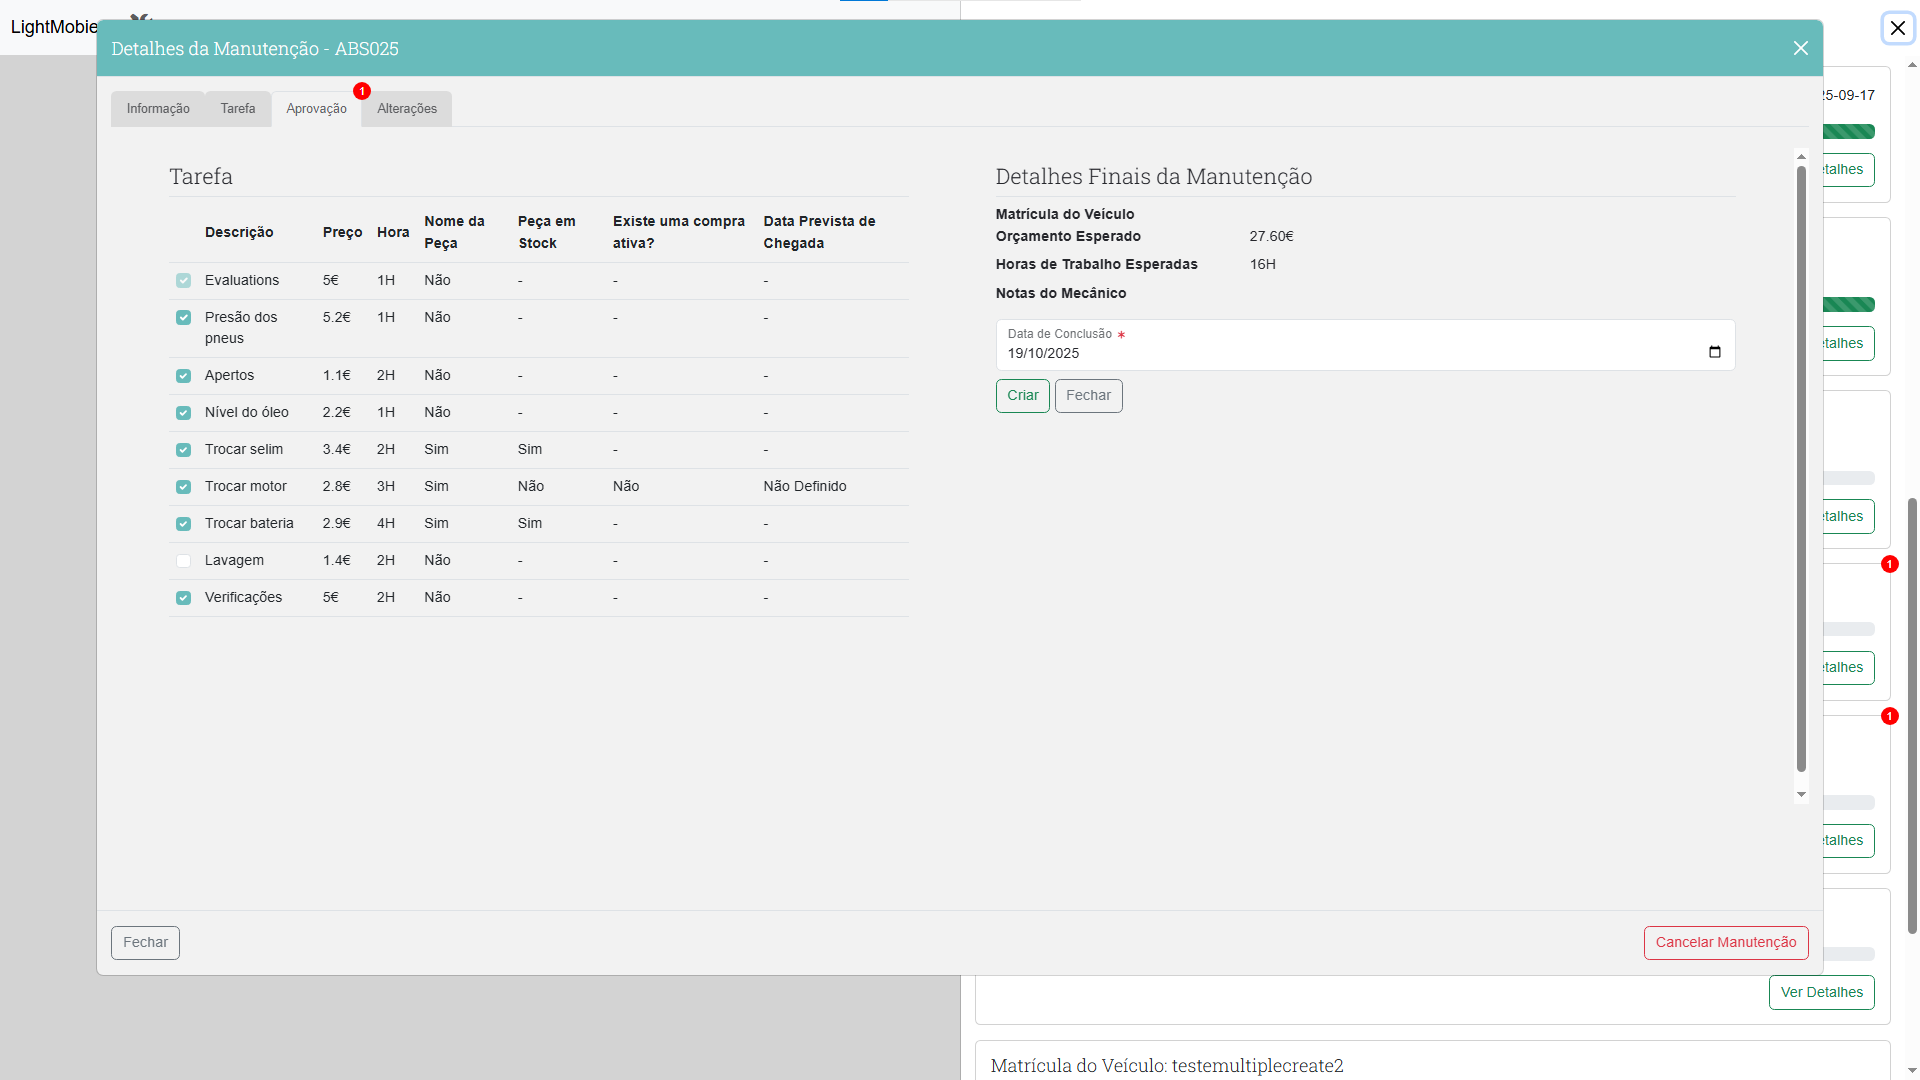
\includegraphics[width=\textwidth]{figs/Implementation/rececionist/maintenance_details_approval}
  \label{fig:impReceMaintApproval}
\end{figure}



Additional features include multilingual support (Portuguese and English) and account management options, allowing the receptionist to switch languages or log out, change email and change password via the profile menu.


\subsection{Mechanic view}


\begin{figure}[h]
  \caption{Mechanic home page with simple, late and previous started task.}
  \centering
  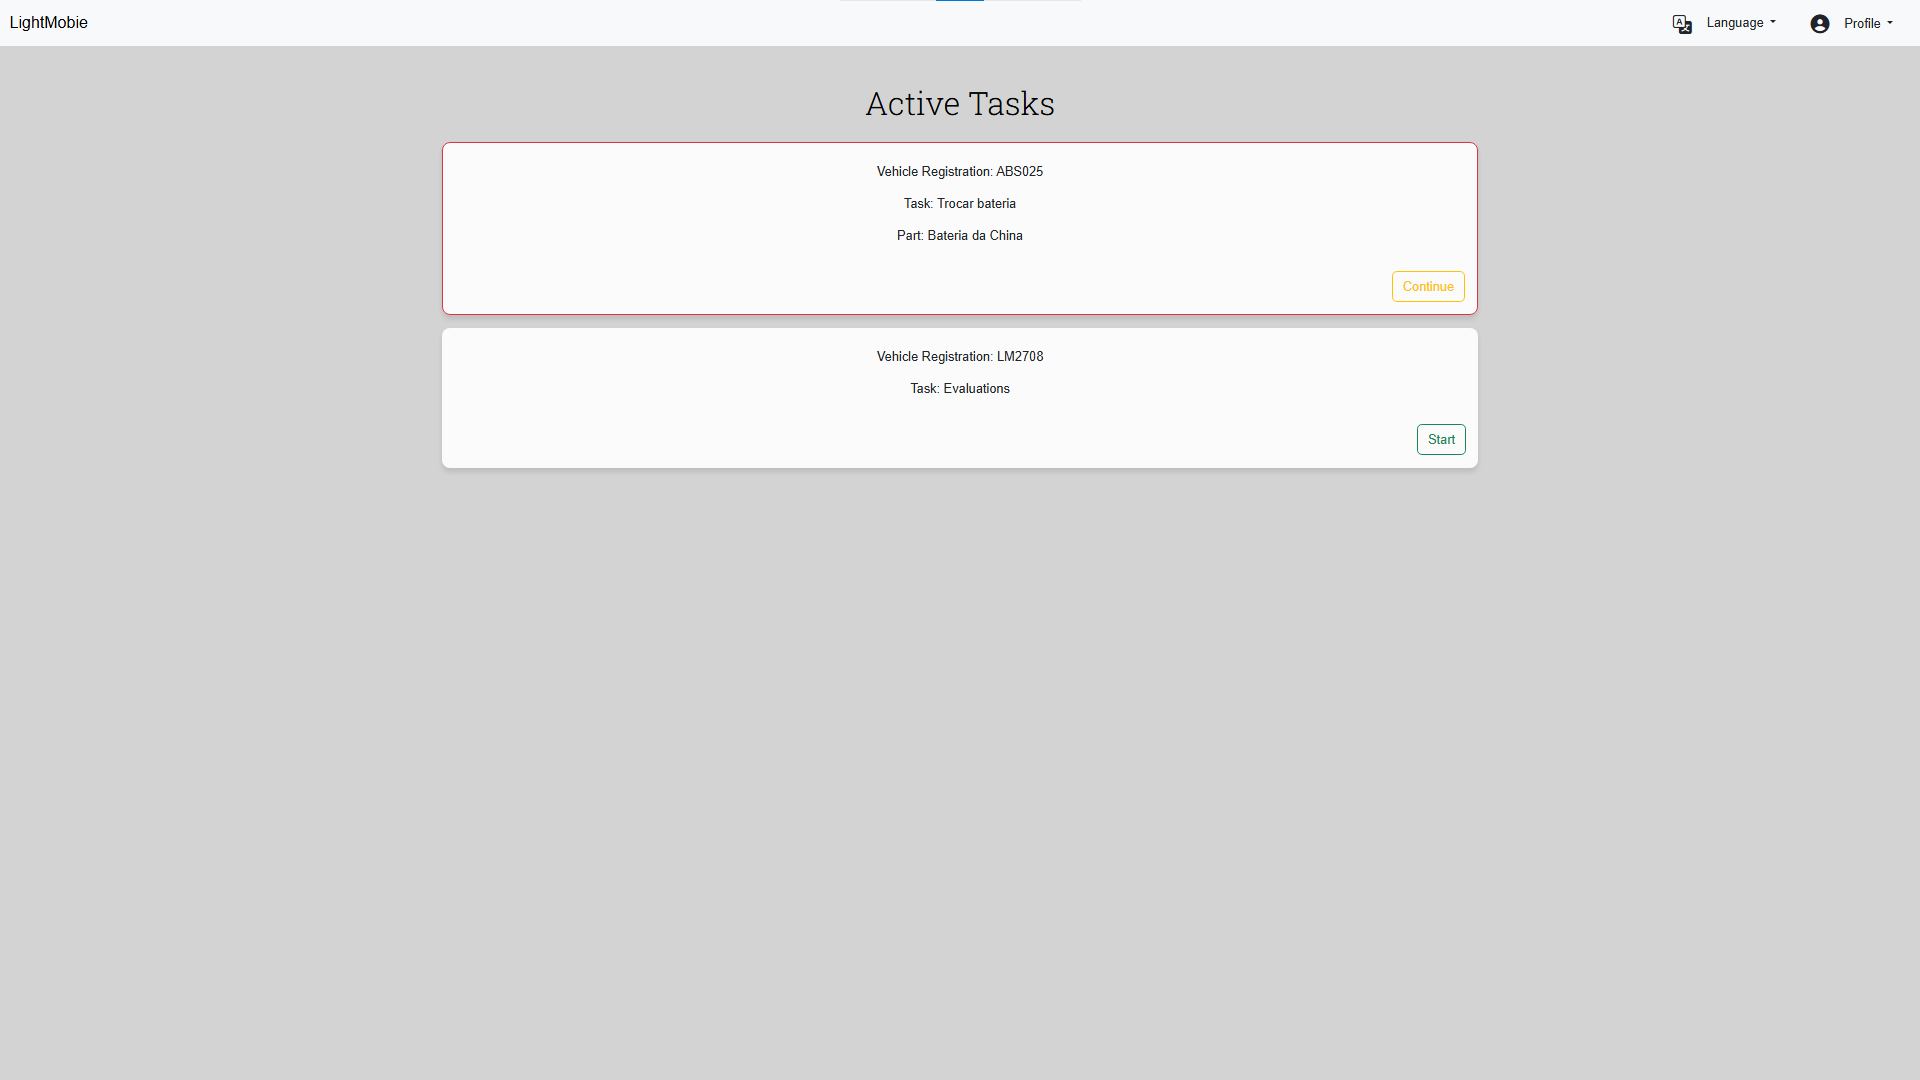
\includegraphics[width=\textwidth]{figs/Implementation/mechanic/HomeShowTasks}
  \label{fig:HomeShowTasks}
\end{figure}





The mechanic interface mirrors the structure of the receptionist's view, but focuses on task execution and vehicle evaluation. On the home page (Figure~\ref{fig:HomeShowTasks}), mechanics can see all tasks assigned to them for the day, including overdue tasks that were started previously but left incomplete. This directly supports Use Case 2.1 – View to-do list and Use Case 2.6 – Continue Task. Each task card provides essential information such as the vehicle registration, task name, and, where applicable, the part required to complete it.



\begin{figure}[h]
  \caption{Vehicle details during a task completion.}
  \centering
  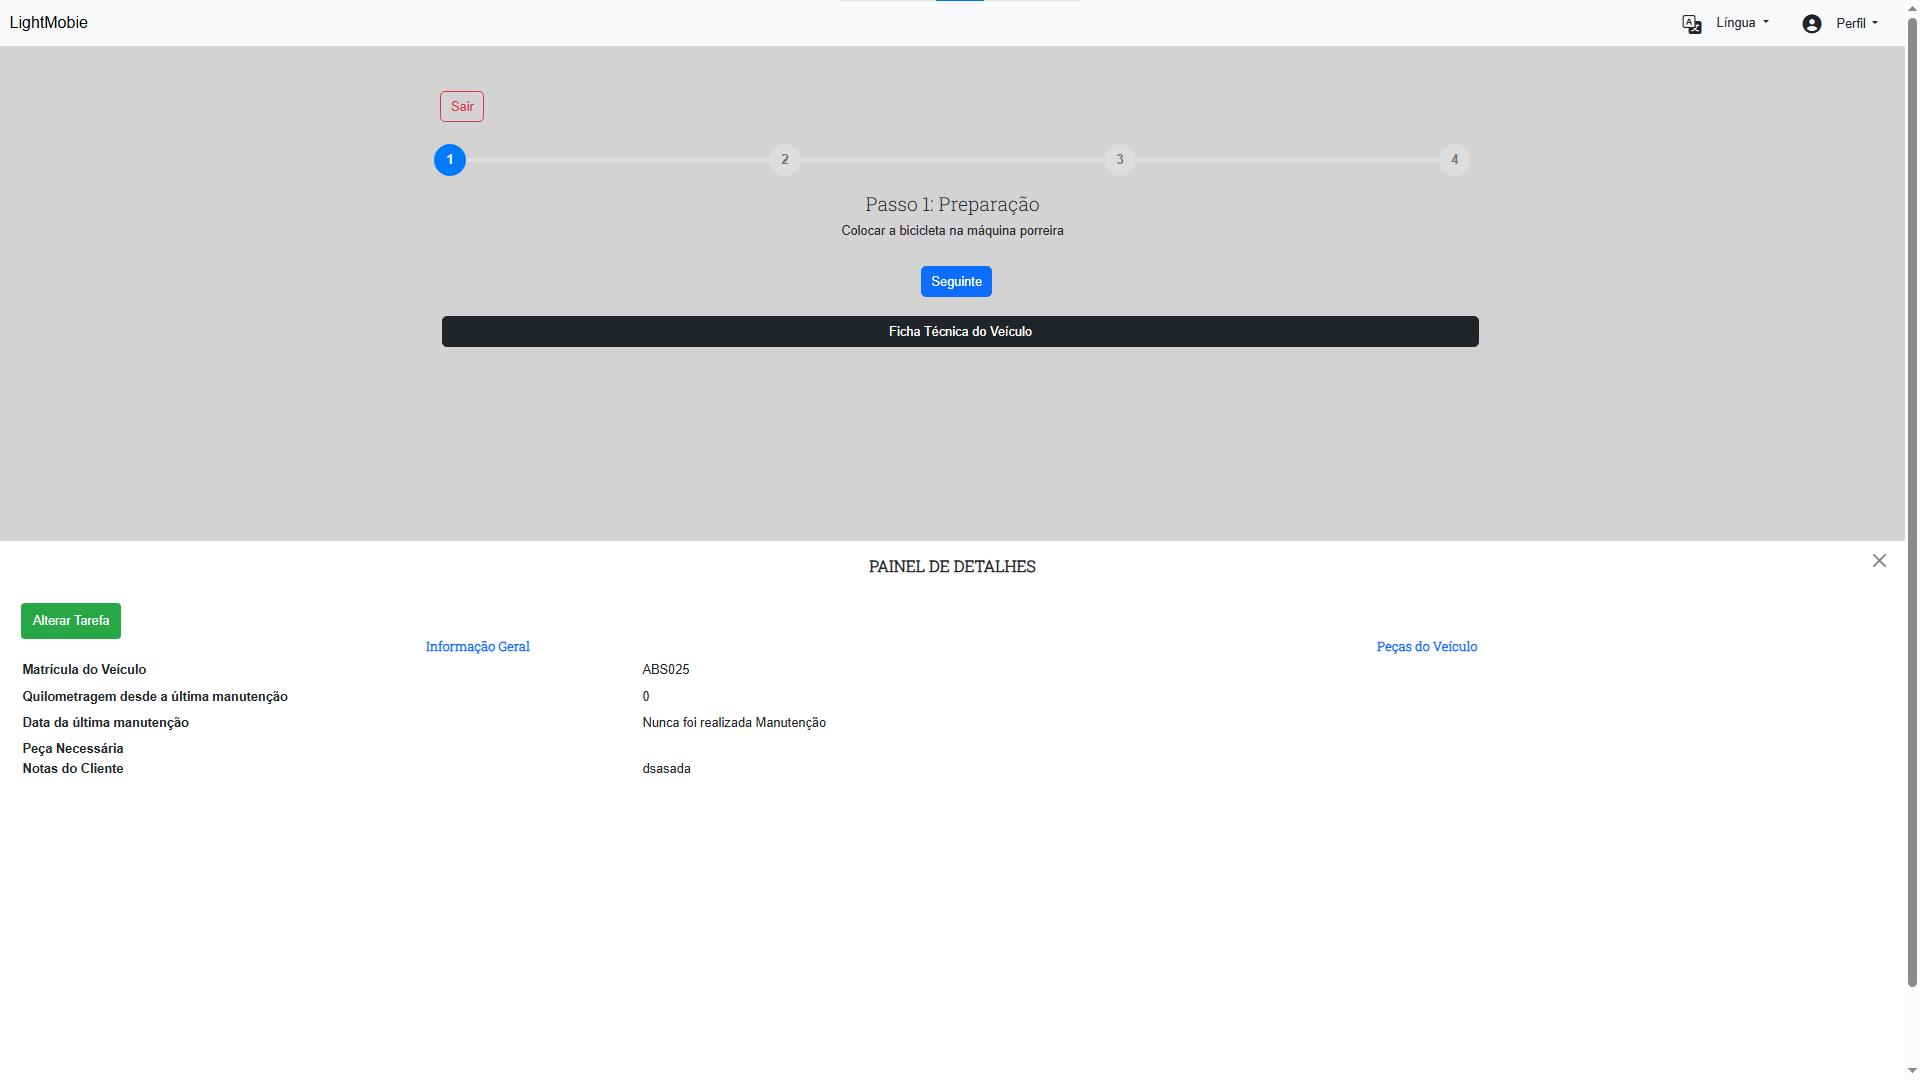
\includegraphics[width=\textwidth]{figs/Implementation/mechanic/MechanicTaskVehicleDetails}
  \label{fig:MechanicTaskVehicleDetails}
\end{figure}



When opening a task, the system guides the mechanic through a series of predefined steps (Figure~\ref{fig:MechanicTaskNormal}). Each step includes instructions, navigation controls, and access to the vehicle's technical details, which can be viewed in an expandable panel (Figure~\ref{fig:MechanicTaskVehicleDetails}). The technical sheet contains registration data, mileage since last maintenance, part history, and any client notes. If, during execution, the mechanic determines that a different part is needed, they may trigger a maintenance change request. This pauses the task, records the proposed modification, and initiates Use Case 2.5 – Change Task (Figure~\ref{fig:MechanicTaskChangeTask}). Once all steps are completed, the mechanic can leave notes and mark the task as finished, fulfilling Use Case 2.4 – Execute Maintenance Task (Figure~\ref{fig:MechanicTaskLastStep}). If the completed task is the final one for the maintenance, the system automatically sends an email notification to the client informing them that the vehicle is ready for pickup, achieving Use Case 5.2 – Receive End Notification (Figure~\ref{fig:MaintenanceFinishedNotification}).




\begin{figure}[h]
  \caption{Mechanic Evaluation first step.}
  \centering
  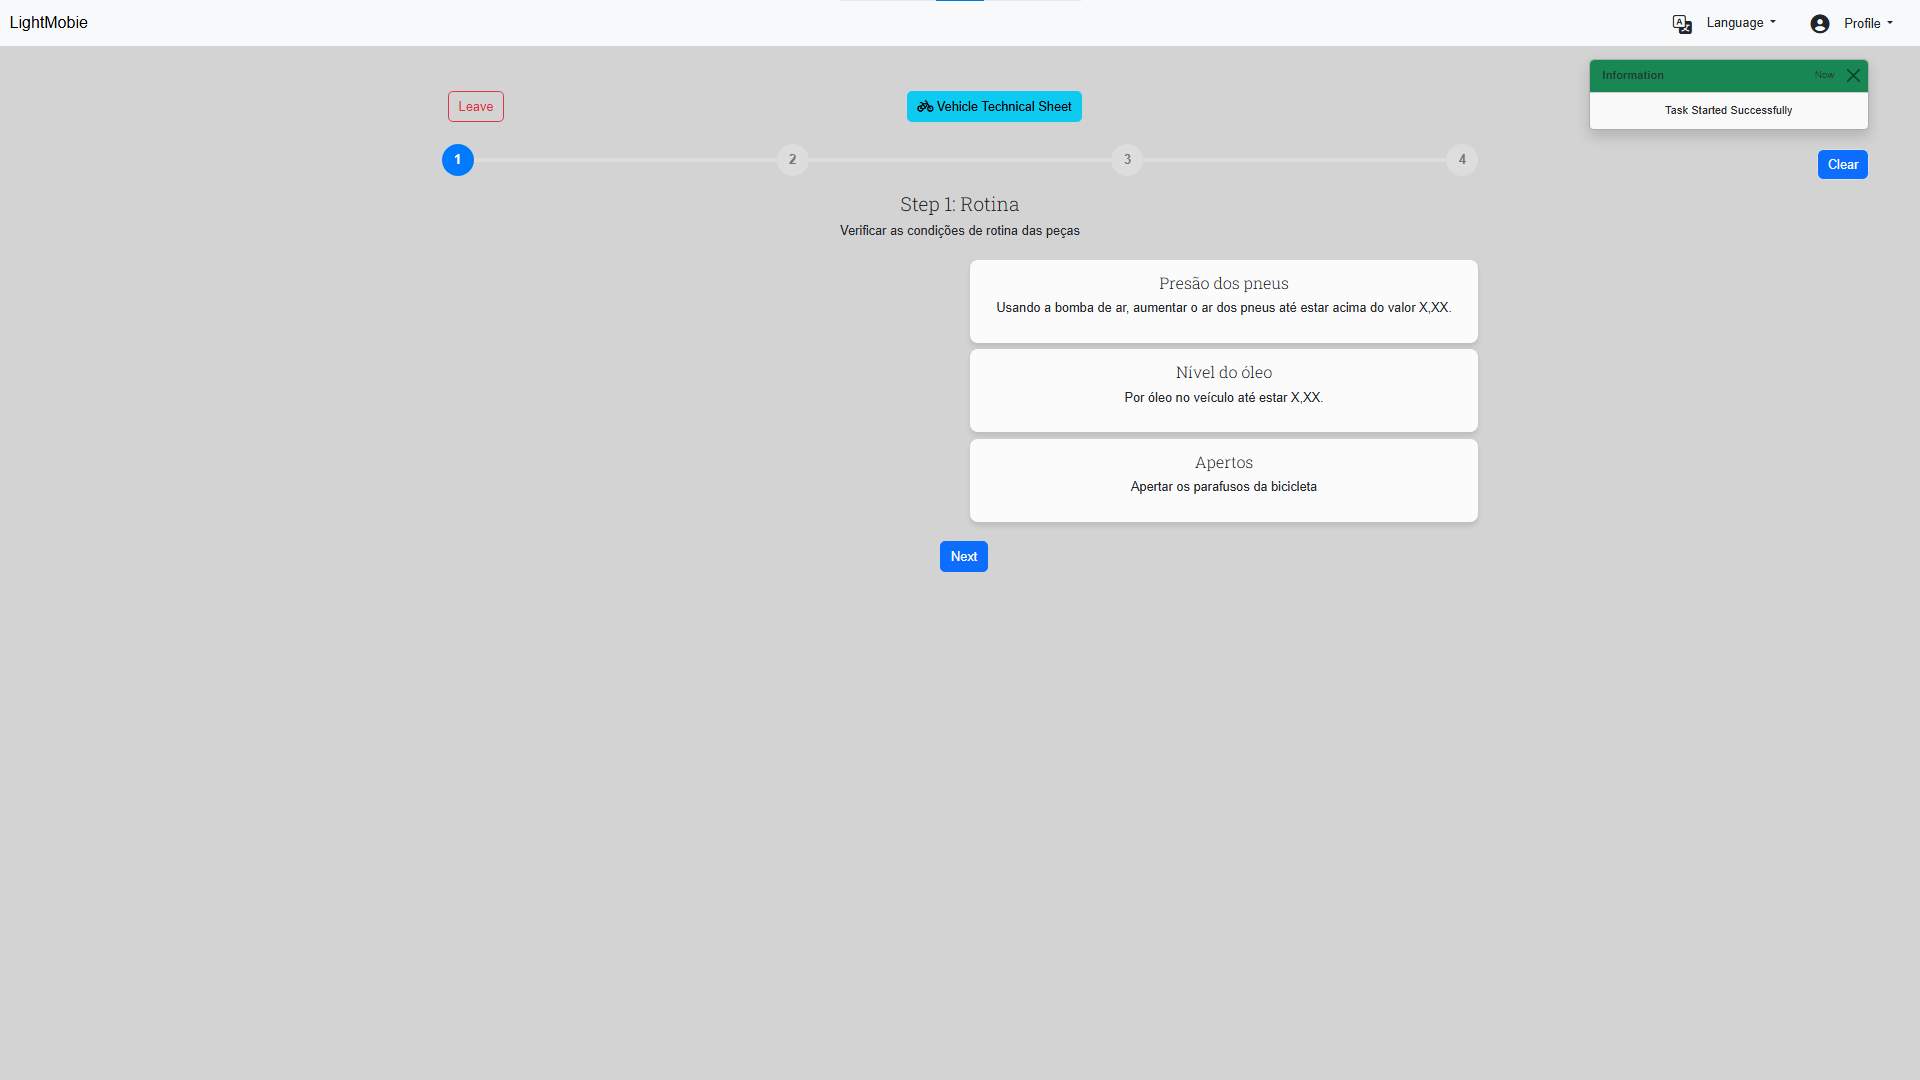
\includegraphics[width=\textwidth]{figs/Implementation/mechanic/MechanicEvaluationNormal}
  \label{fig:MechanicEvaluationNormal}
\end{figure}





The interface also supports vehicle evaluations, where the mechanic identifies and registers new tasks (Figures~\ref{fig:MechanicEvaluationSelectTaskWitPart}-~\ref{fig:TaskSelected}). Starting an evaluation presents a list of potential tasks, each of which can be selected and, if necessary, linked to specific parts. The system checks warehouse stock levels in real time, alerting the mechanic if parts are unavailable so adjustments can be made. Selected tasks are visually highlighted, providing immediate feedback. In the final step of the evaluation (Figure~\ref{fig:EvaluationLastStep}), the mechanic reviews the chosen tasks and records the cause of each anomaly before submitting. Completing this workflow corresponds to Use Case 2.2 – Carry out a vehicle analysis or Use Case 2.3 – Register completed tasks, depending on whether the dealership configuration.


\subsection{Warehouse Operator view}


\begin{figure}[h]
  \caption{Warehouse home page.}
  \centering
  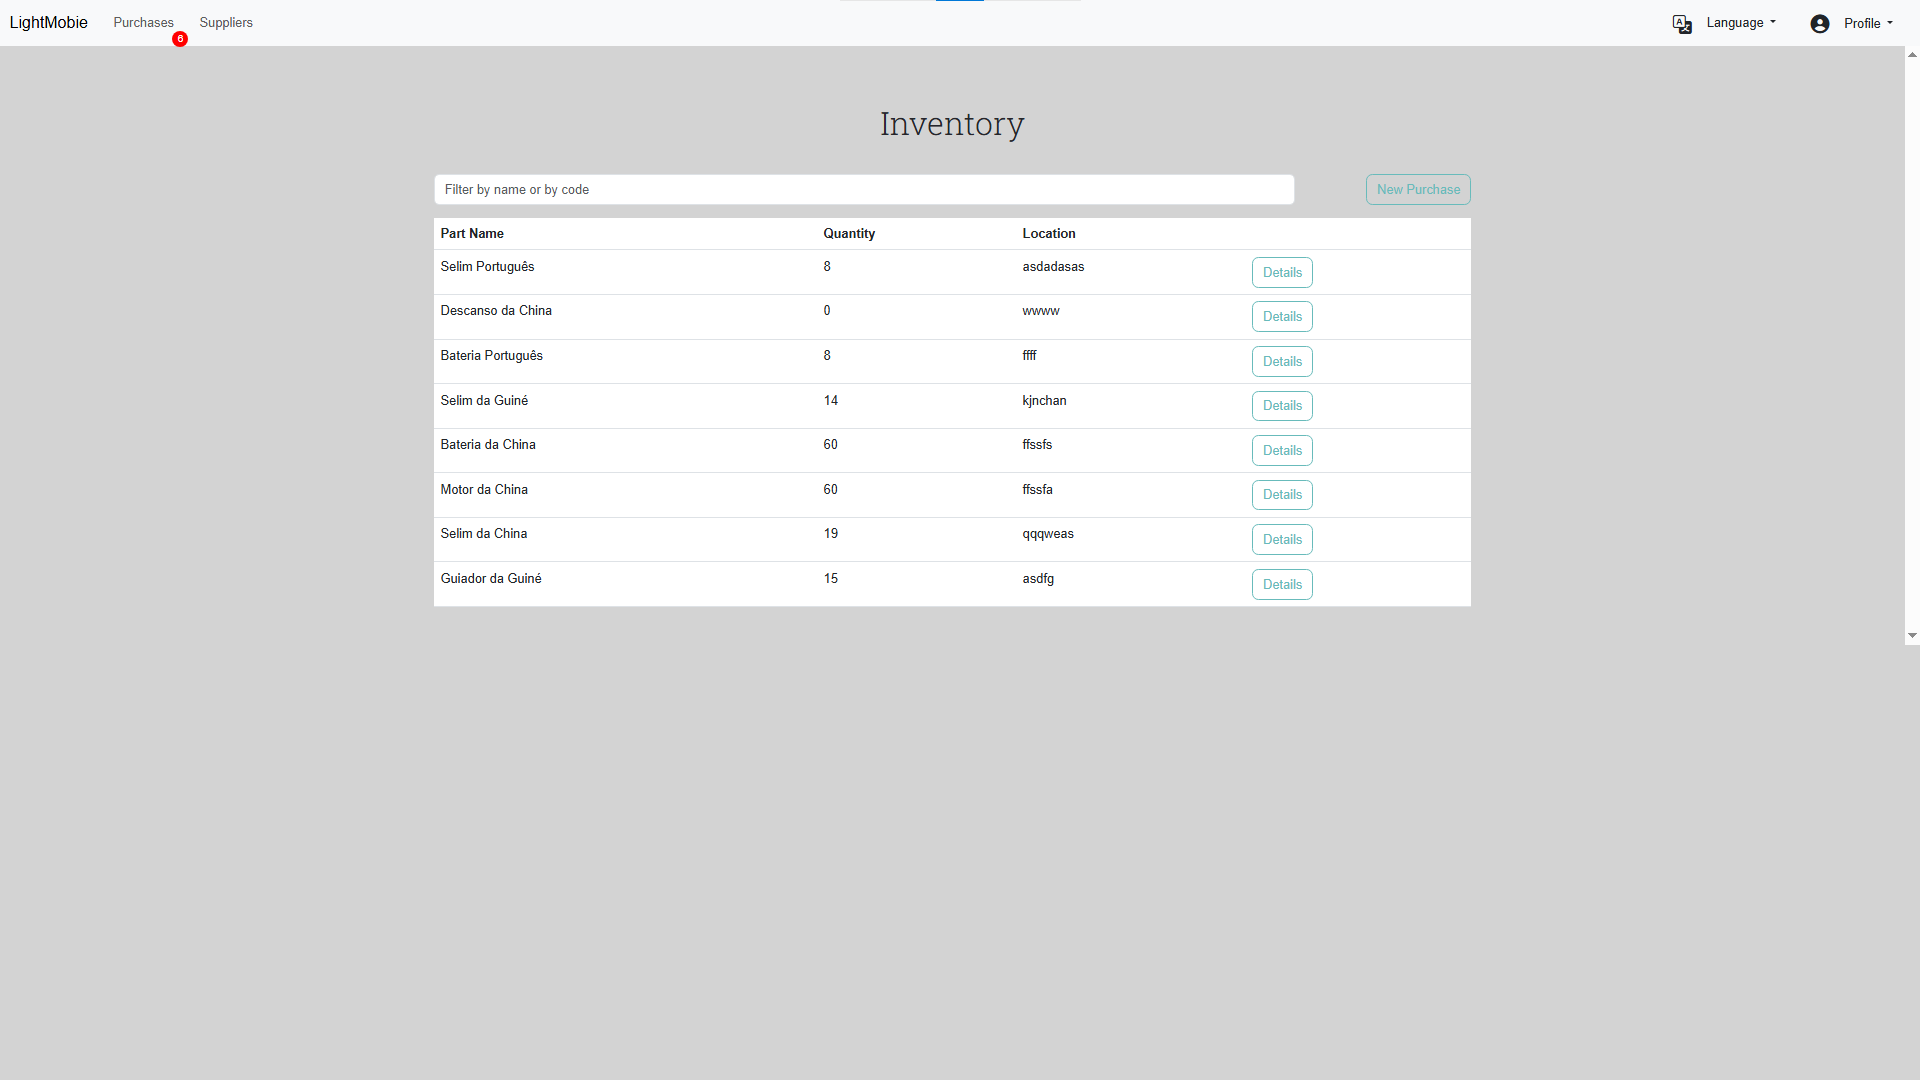
\includegraphics[width=\textwidth]{figs/Implementation/warehouse/homepage}
  \label{fig:warehouseHomepage}
\end{figure}



The warehouse operator interface follows the same overall layout as the other views, with a top menu and a central workspace (Figure~\ref{fig:warehouseHomepage}). Its primary purpose is to manage parts inventory, handle purchase requests, and maintain supplier information, covering all operations in Use Case Group 3.


\begin{figure}[h]
  \caption{Inventory details.}
  \centering
  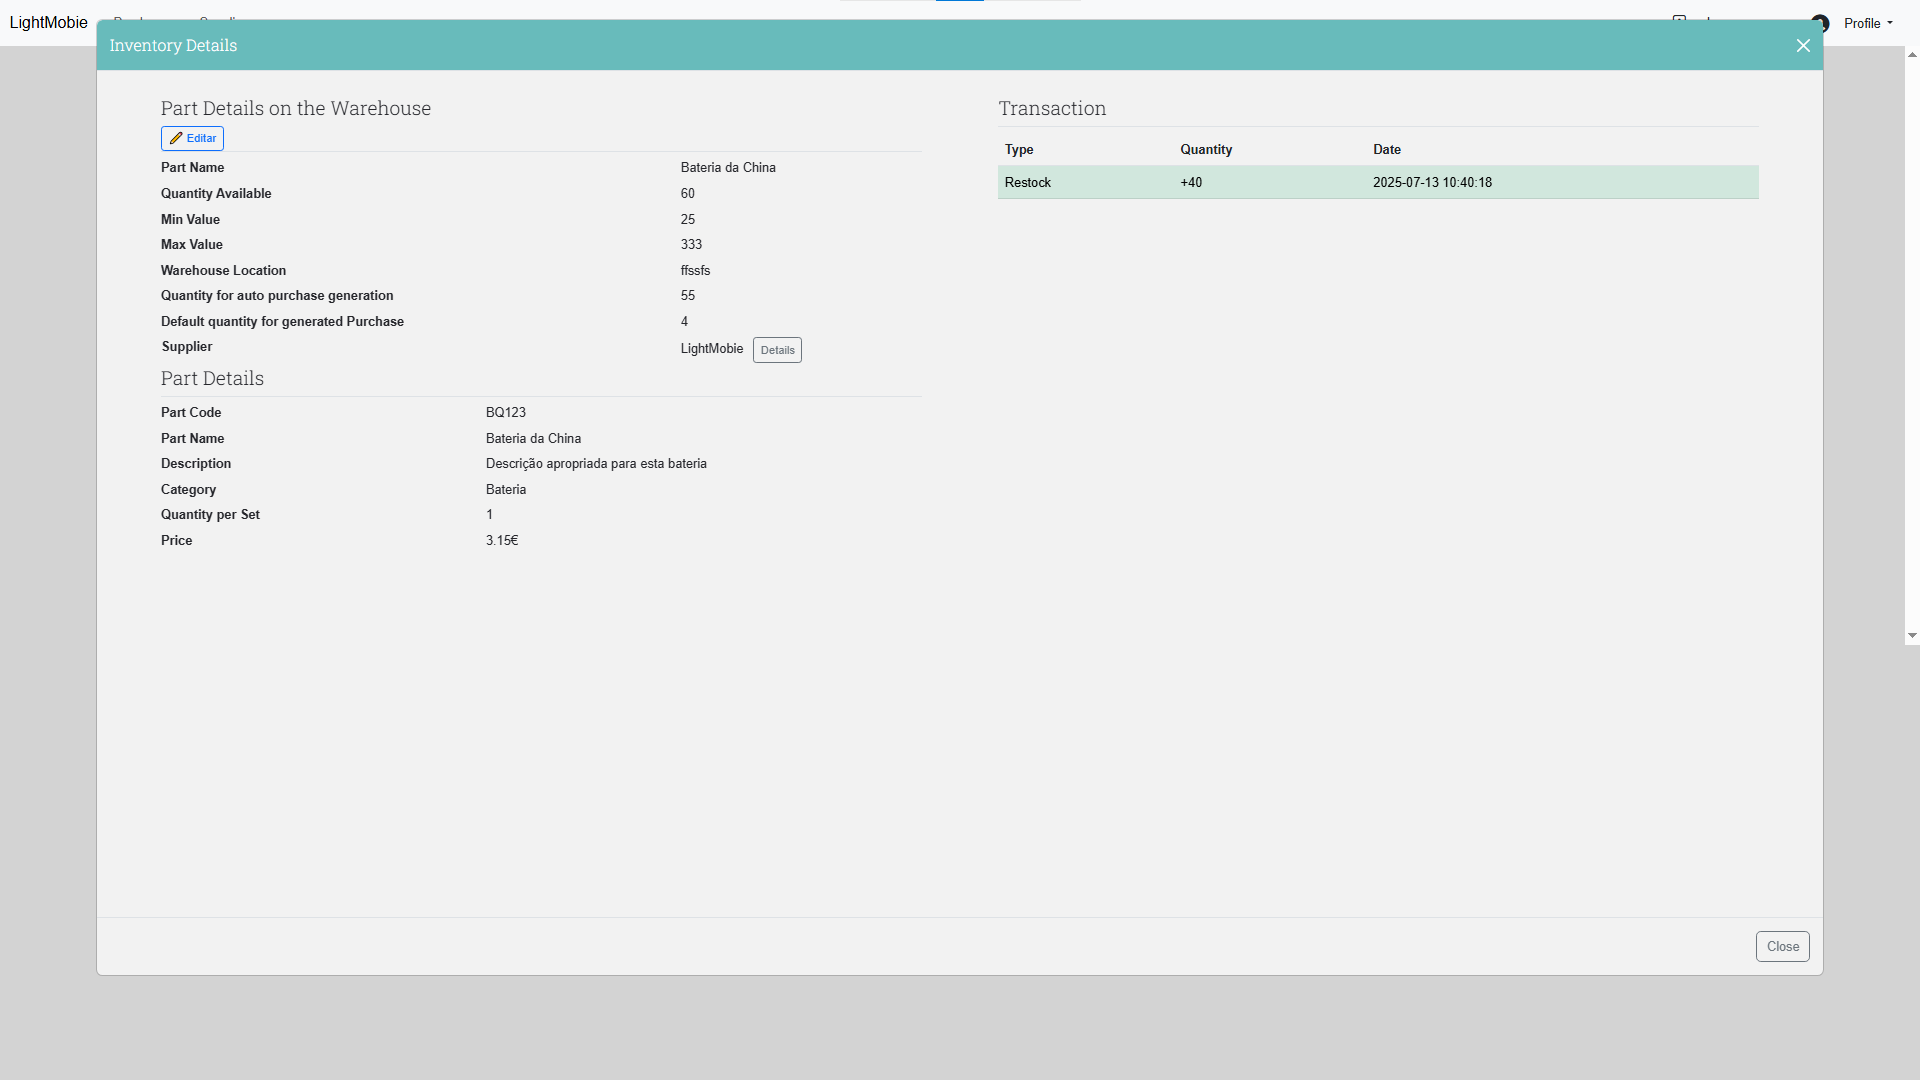
\includegraphics[width=\textwidth]{figs/Implementation/warehouse/inventoryDetails}
  \label{fig:inventoryDetails}
\end{figure}


The inventory section presents a searchable table of all parts stored in the warehouse, including their available quantity and location code (Use Case 3.1 – View warehouse parts). Each entry can be expanded to display detailed information such as stock thresholds, purchase configuration parameters, transaction history, and pricing (Figure~\ref{fig:inventoryDetails}). Operators can also edit inventory settings—such as location, minimum and maximum stock levels, and automatic purchase triggers—fulfilling Use Case 3.5 – Edit inventory (Figure~\ref{fig:inventoryEdit}).


\begin{figure}[h]
  \caption{Create new purchase modal.}
  \centering
  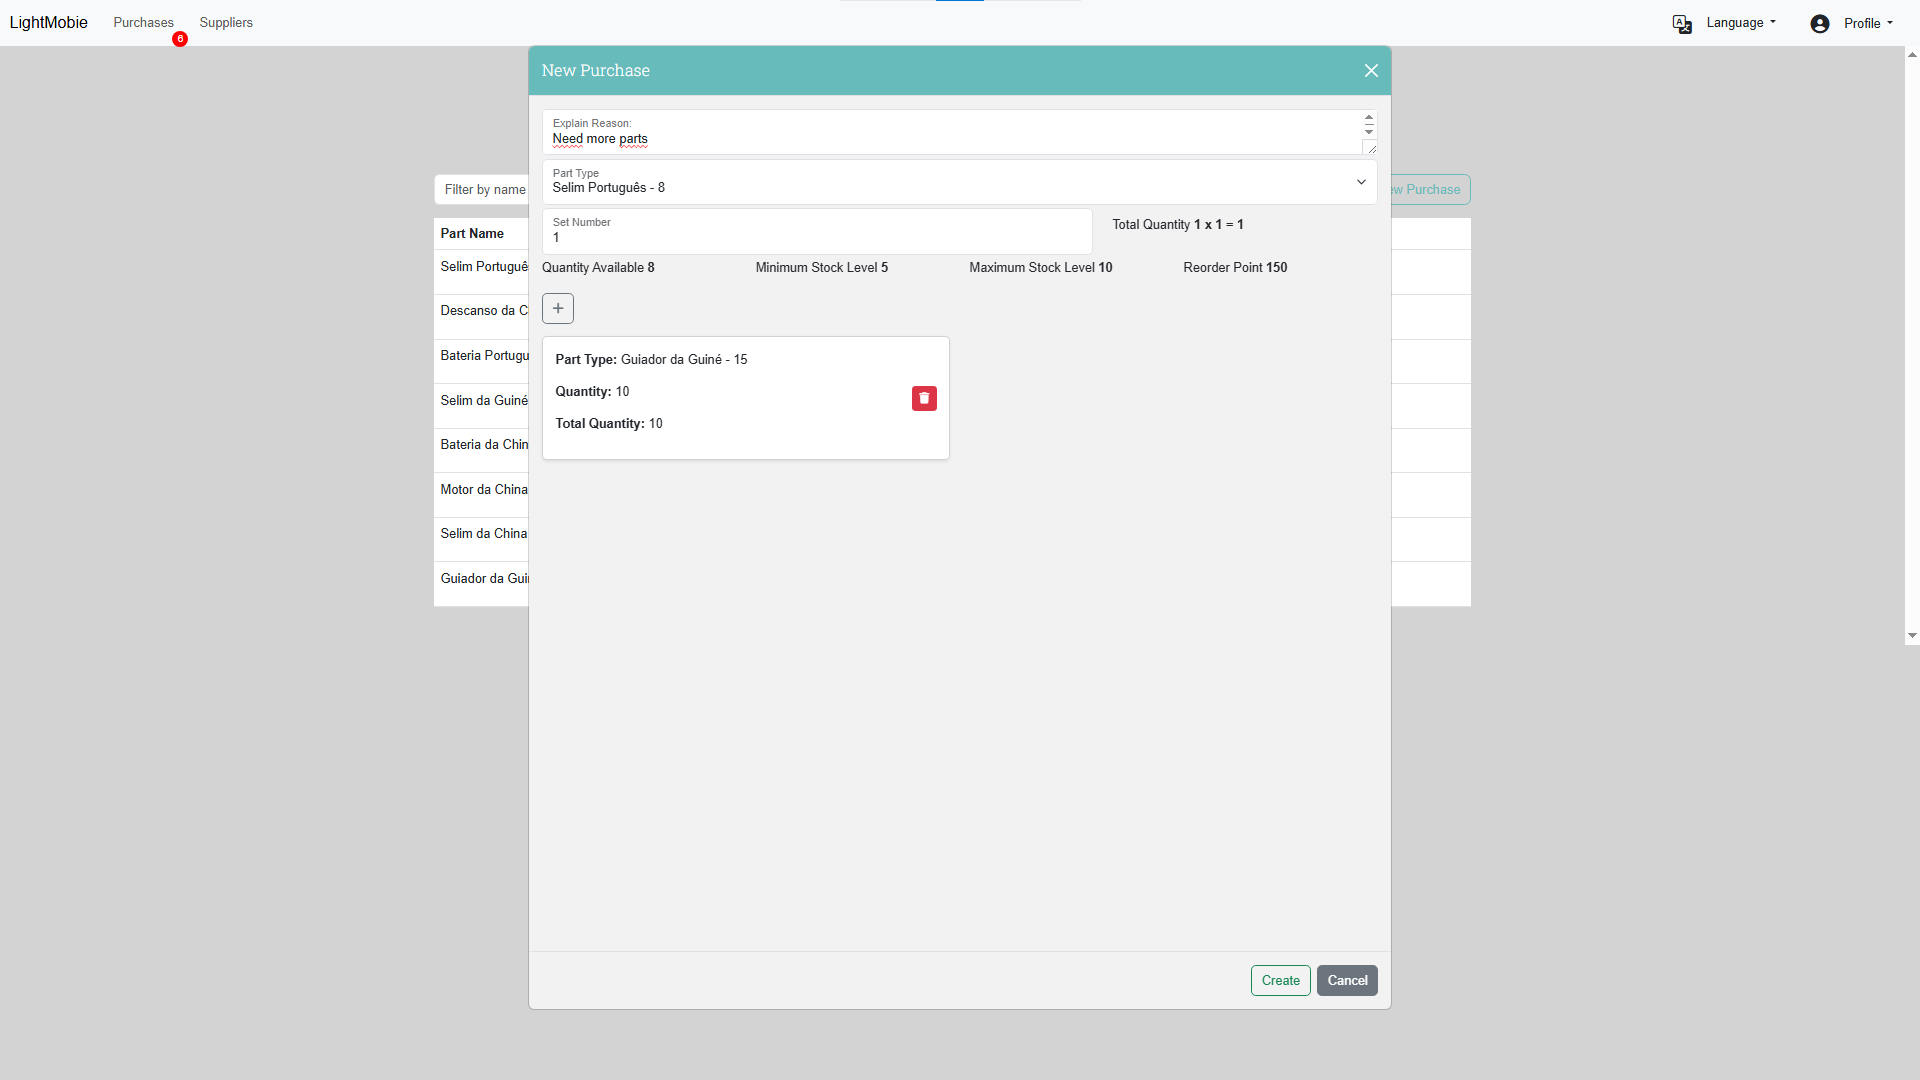
\includegraphics[width=\textwidth]{figs/Implementation/warehouse/createPurchase}
  \label{fig:createPurchase}
\end{figure}


\begin{figure}[h]
  \caption{List of purchases.}
  \centering
  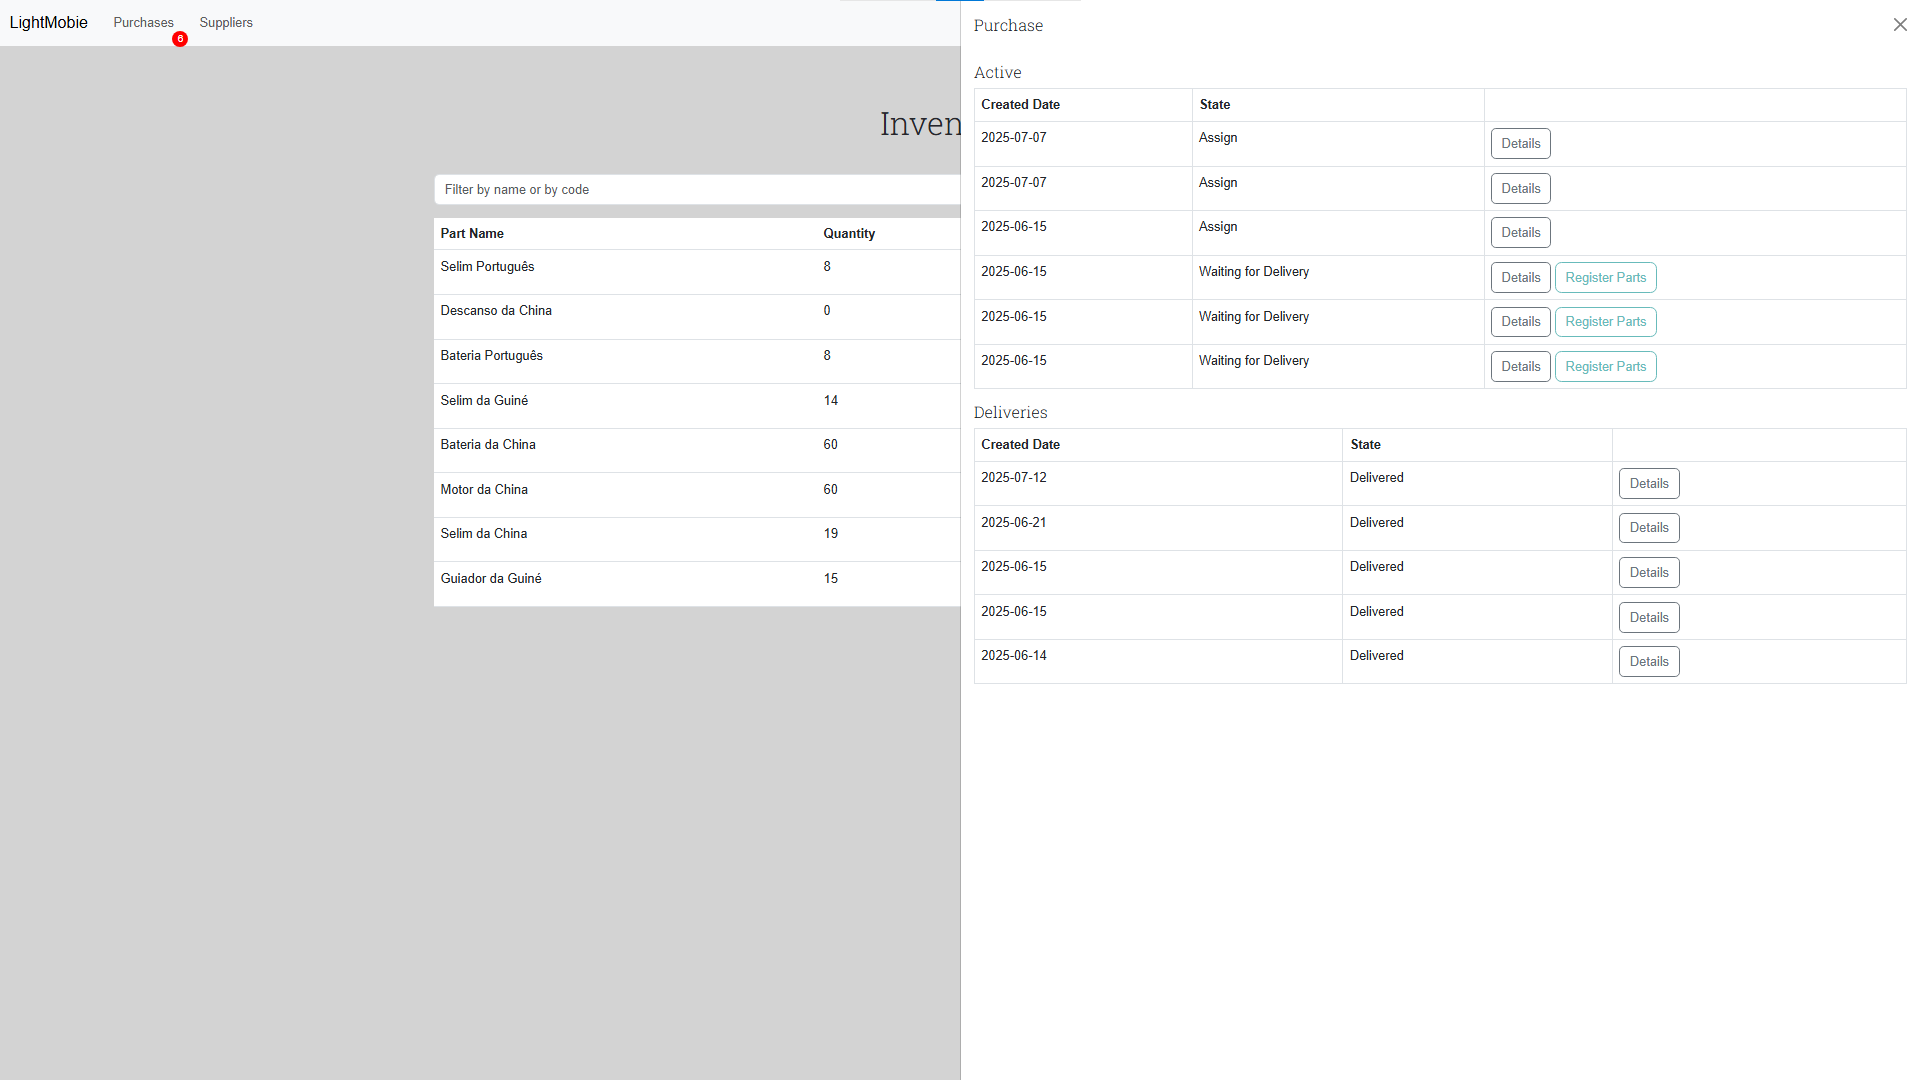
\includegraphics[width=\textwidth]{figs/Implementation/warehouse/PurchaseList}
  \label{fig:PurchaseList}
\end{figure}






Purchases are managed directly from the home page. Operators may create new purchase requests by specifying a justification and selecting parts and quantities (Figures~\ref{fig:createPurchase}), which initiates Use Case 3.2 – Request purchasing service. All purchases are accessible from a dedicated view, where they are organized by status: assigned, awaiting delivery, or completed (Figure~\ref{fig:PurchaseList}). Assigned purchases allow operators to review order details and record expected arrival dates (Figure~\ref{fig:PurchaseDetails}). Waiting delivery purchases support both delaying arrivals (Use Case 3.6 – Create purchase delay) and registering the reception of parts (Use Case 3.4 – Register new parts in the system) (Figure~\ref{fig:PurchaseRegisterParts}). Delivered purchases remain available for reference (Figure~\ref{fig:PurchaseFinishedDetails}).


\begin{figure}[h]
  \caption{Supplier list.}
  \centering
  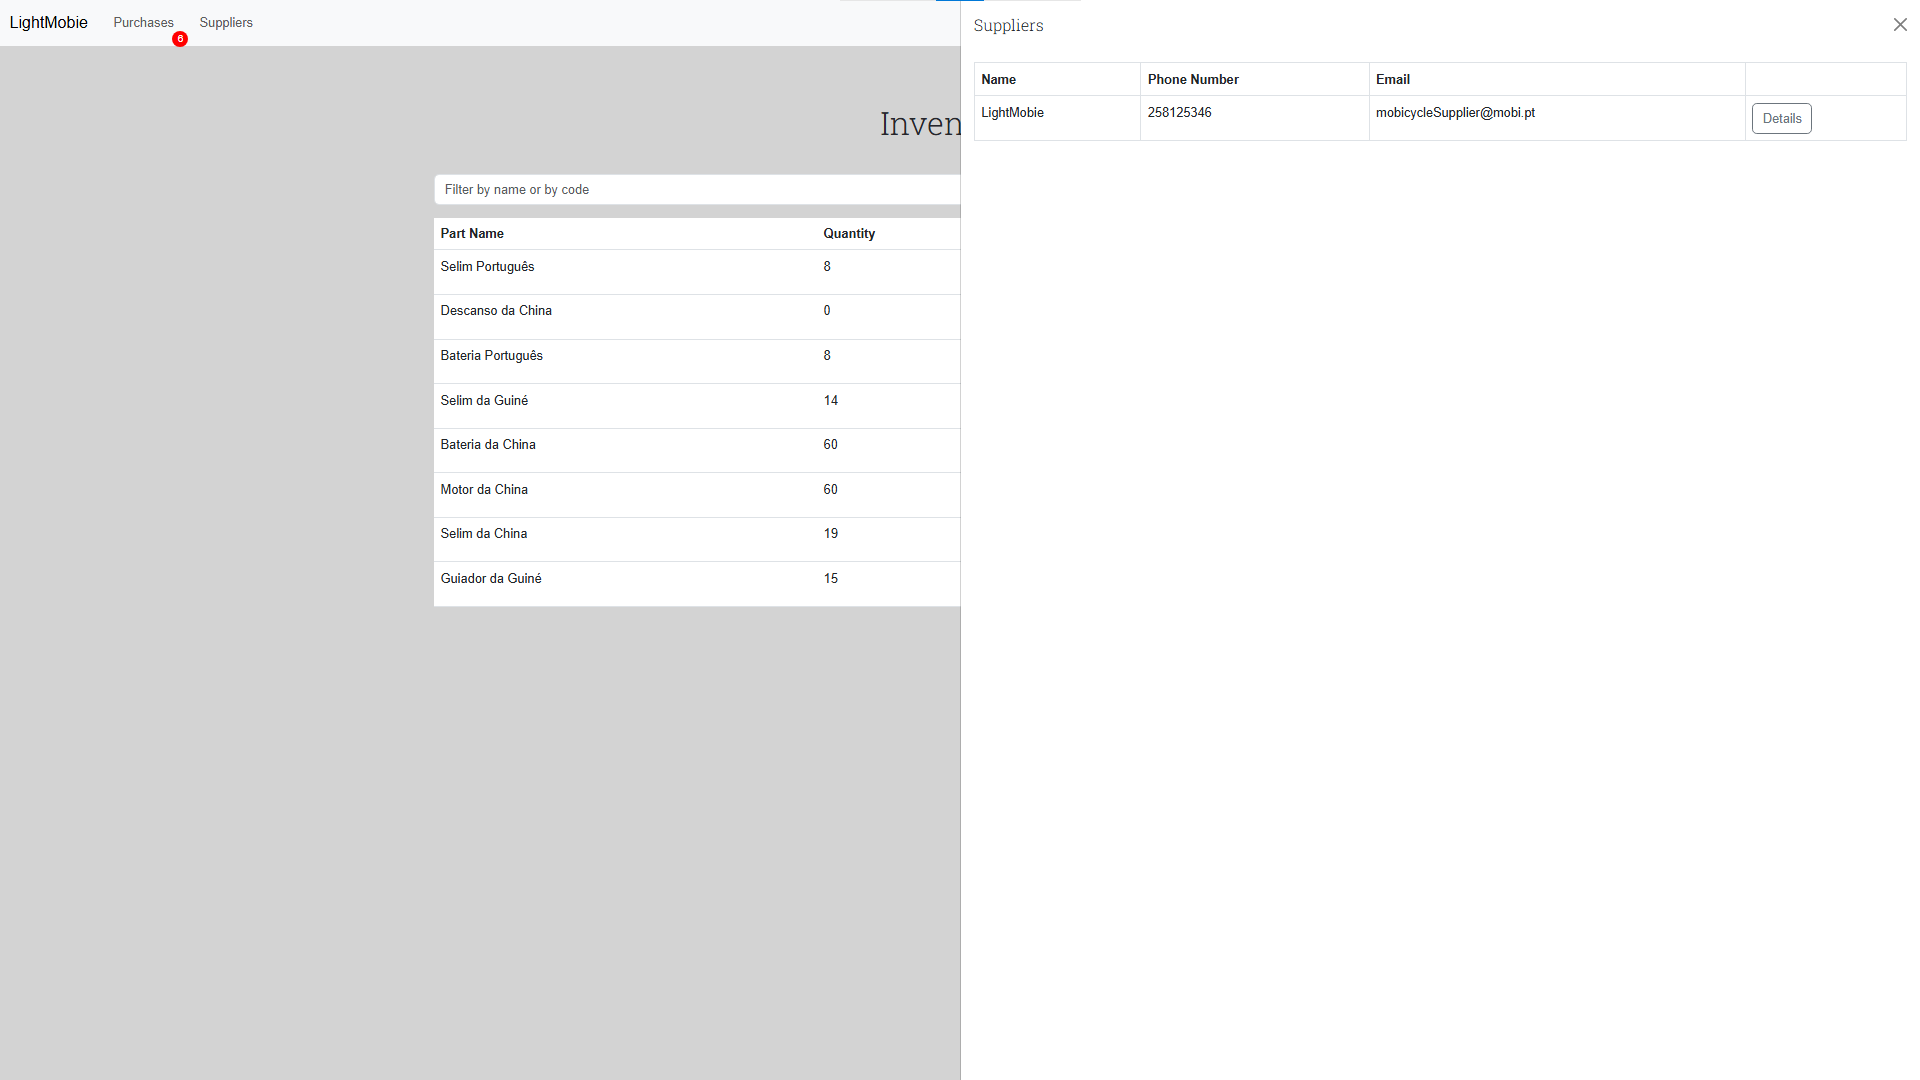
\includegraphics[width=\textwidth]{figs/Implementation/warehouse/supplierList}
  \label{fig:supplierList}
\end{figure}



Finally, the supplier management module enables operators to view and maintain supplier information. A dedicated view lists all suppliers with their contact details (Figure~\ref{fig:supplierList}). Selecting a supplier provides extended information, including address, supplied parts, and contract duration (Figure~\ref{fig:supplierDetails}). This functionality ensures that purchase negotiations and supplier relations remain transparent and up to date.

\subsection{Workshop Manager view}


The workshop manager interface serves as the central hub for overseeing dealership operations. Its layout is consistent with the other views, but it integrates features from both the receptionist and warehouse operator roles, reflecting the manager's broader responsibilities.


\begin{figure}[h]
  \caption{Workshop manager home page.}
  \centering
  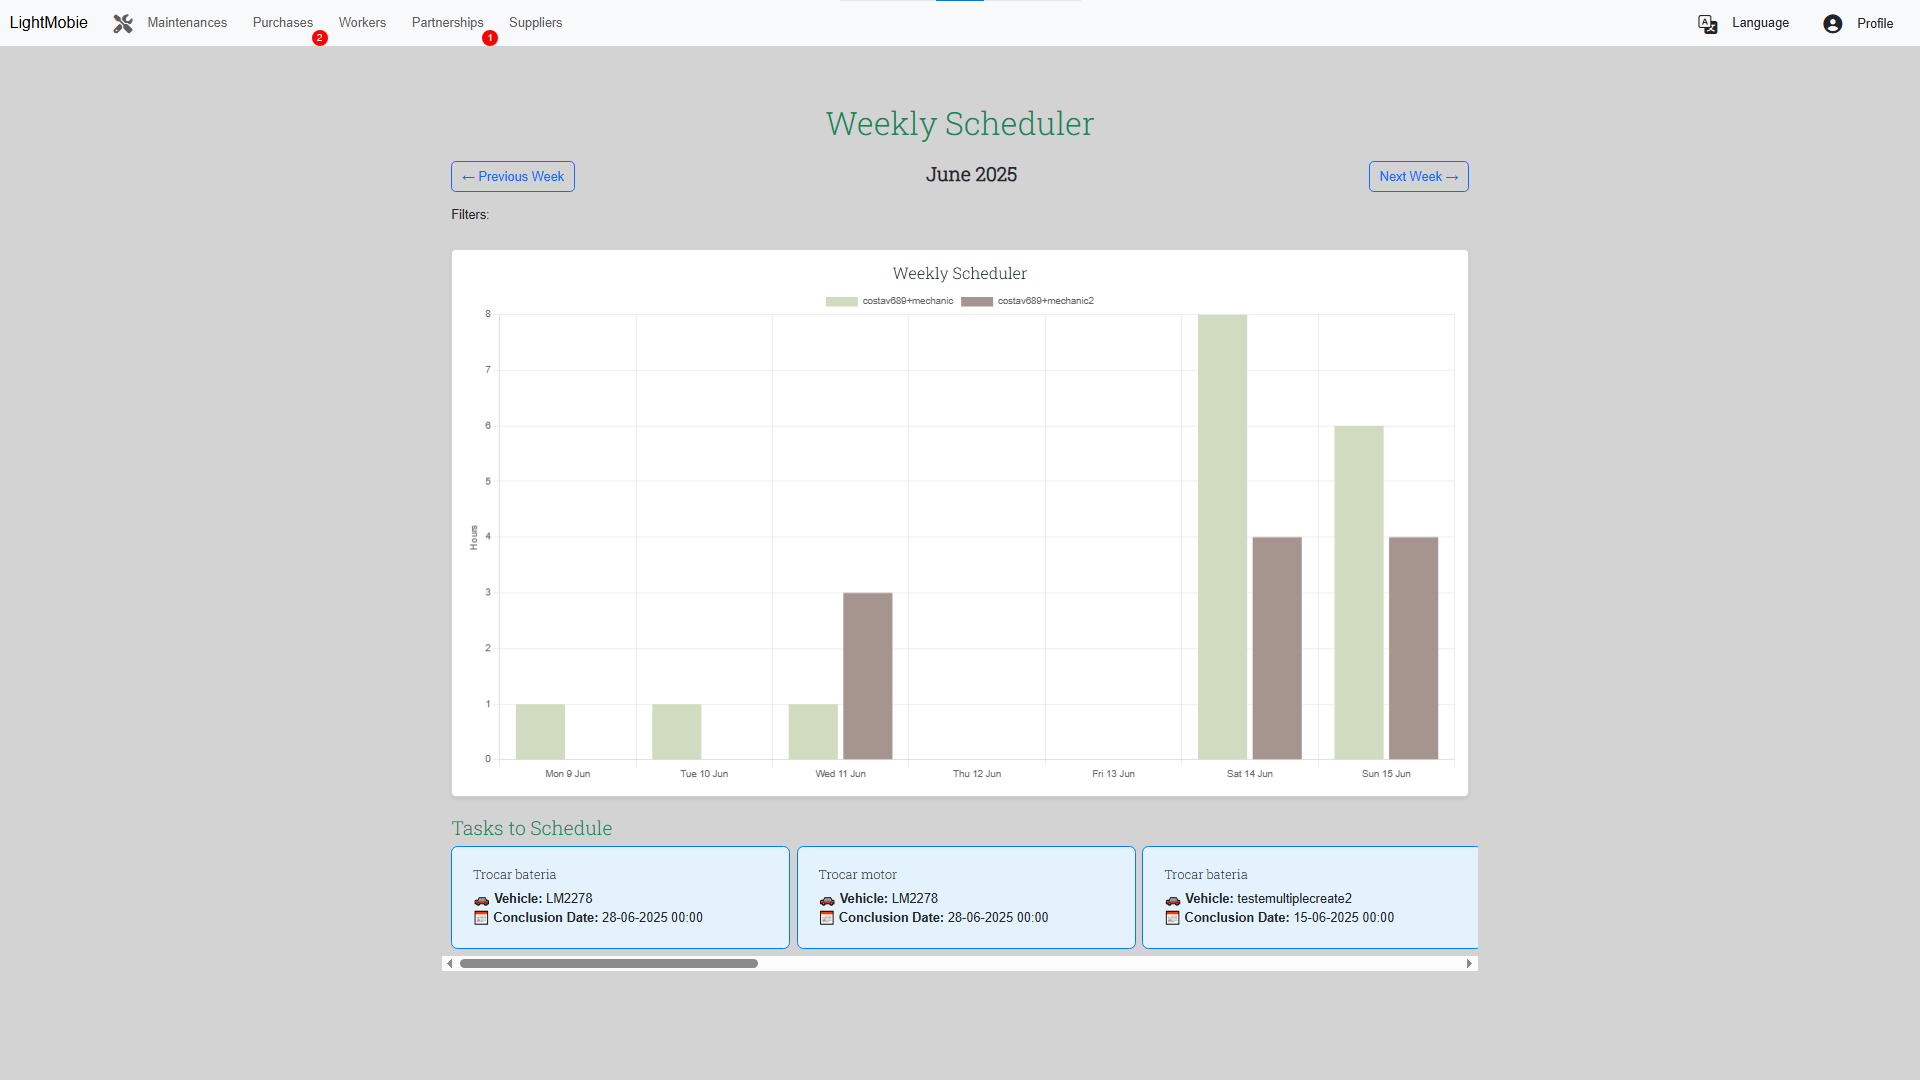
\includegraphics[width=\textwidth]{figs/Implementation/workshopmanager/homePage}
  \label{fig:workshopmanagerHomePage}
\end{figure}



The home page presents a weekly overview of mechanic tasks (Figure~\ref{fig:workshopmanagerHomePage}). Unlike the receptionist's schedule, it highlights unassigned tasks, which the manager can allocate to mechanics, fulfilling Use Case 4.1 – Assign tasks. This can be done either directly from the schedule or by opening a task assignment modal (Figure~\ref{fig:workshopmanagerAssignTask}).






\begin{figure}[h]
  \caption{Maintenance history list.}
  \centering
  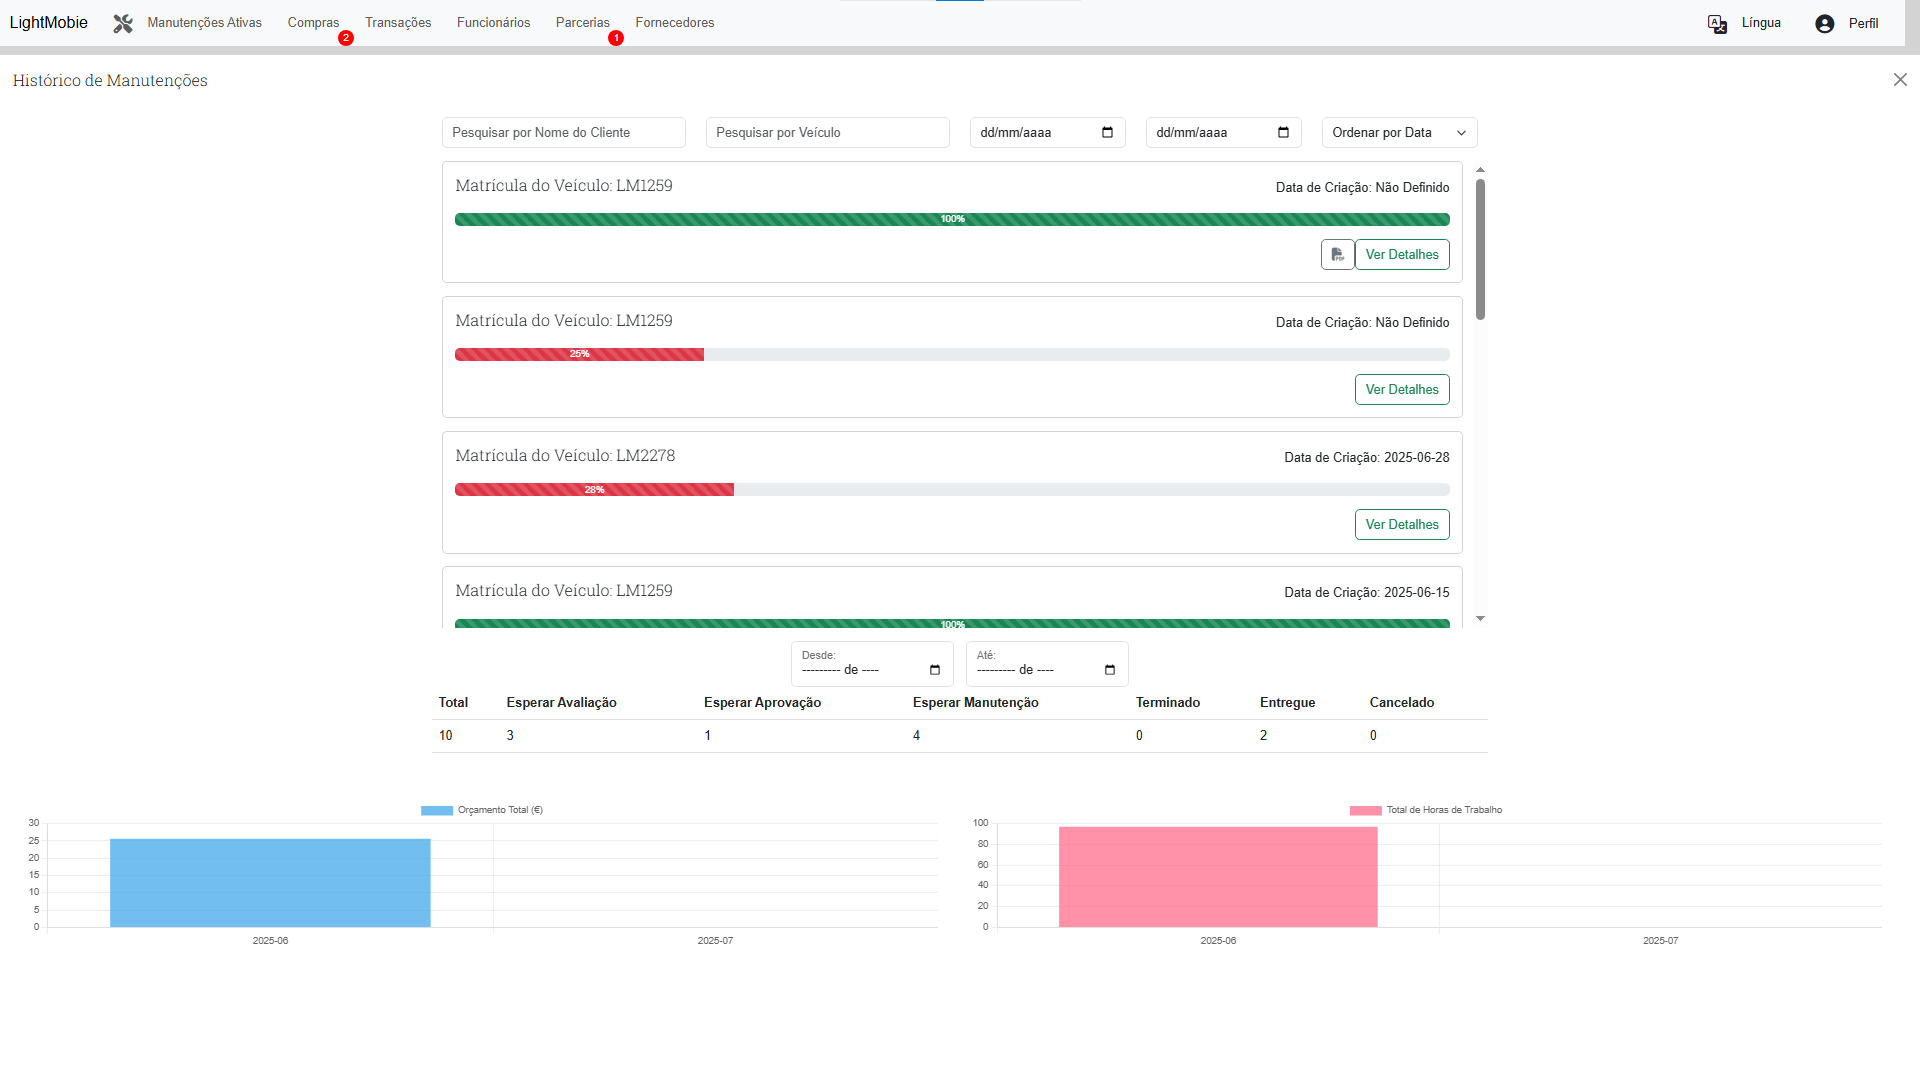
\includegraphics[width=\textwidth]{figs/Implementation/workshopmanager/maintenanceHistory}
  \label{fig:maintenanceHistory}
\end{figure}



Maintenance management mirrors the receptionist's view: active maintenances are listed with their details and task breakdowns (Figures~\ref{fig:workshopmanagerMaintenanceList}-~\ref{fig:workshopmanagerMaintenanceDetailsTask}). The key distinction is that the manager can add new tasks to an ongoing maintenance, which triggers a client validation process. In addition, the manager has access to the maintenance history, supporting Use Case 4.3 – View history of maintenance performed. Past maintenances can be filtered by client, vehicle, or date, and completed cases allow generating PDF reports (Figures~\ref{fig:maintenanceHistory} and ~\ref{fig:report}). Below the history list, statistics such as revenue and working hours are displayed, corresponding to Use Case 4.4 – Develop statistics.

\begin{figure}[h]
  \caption{Purchase request list.}
  \centering
  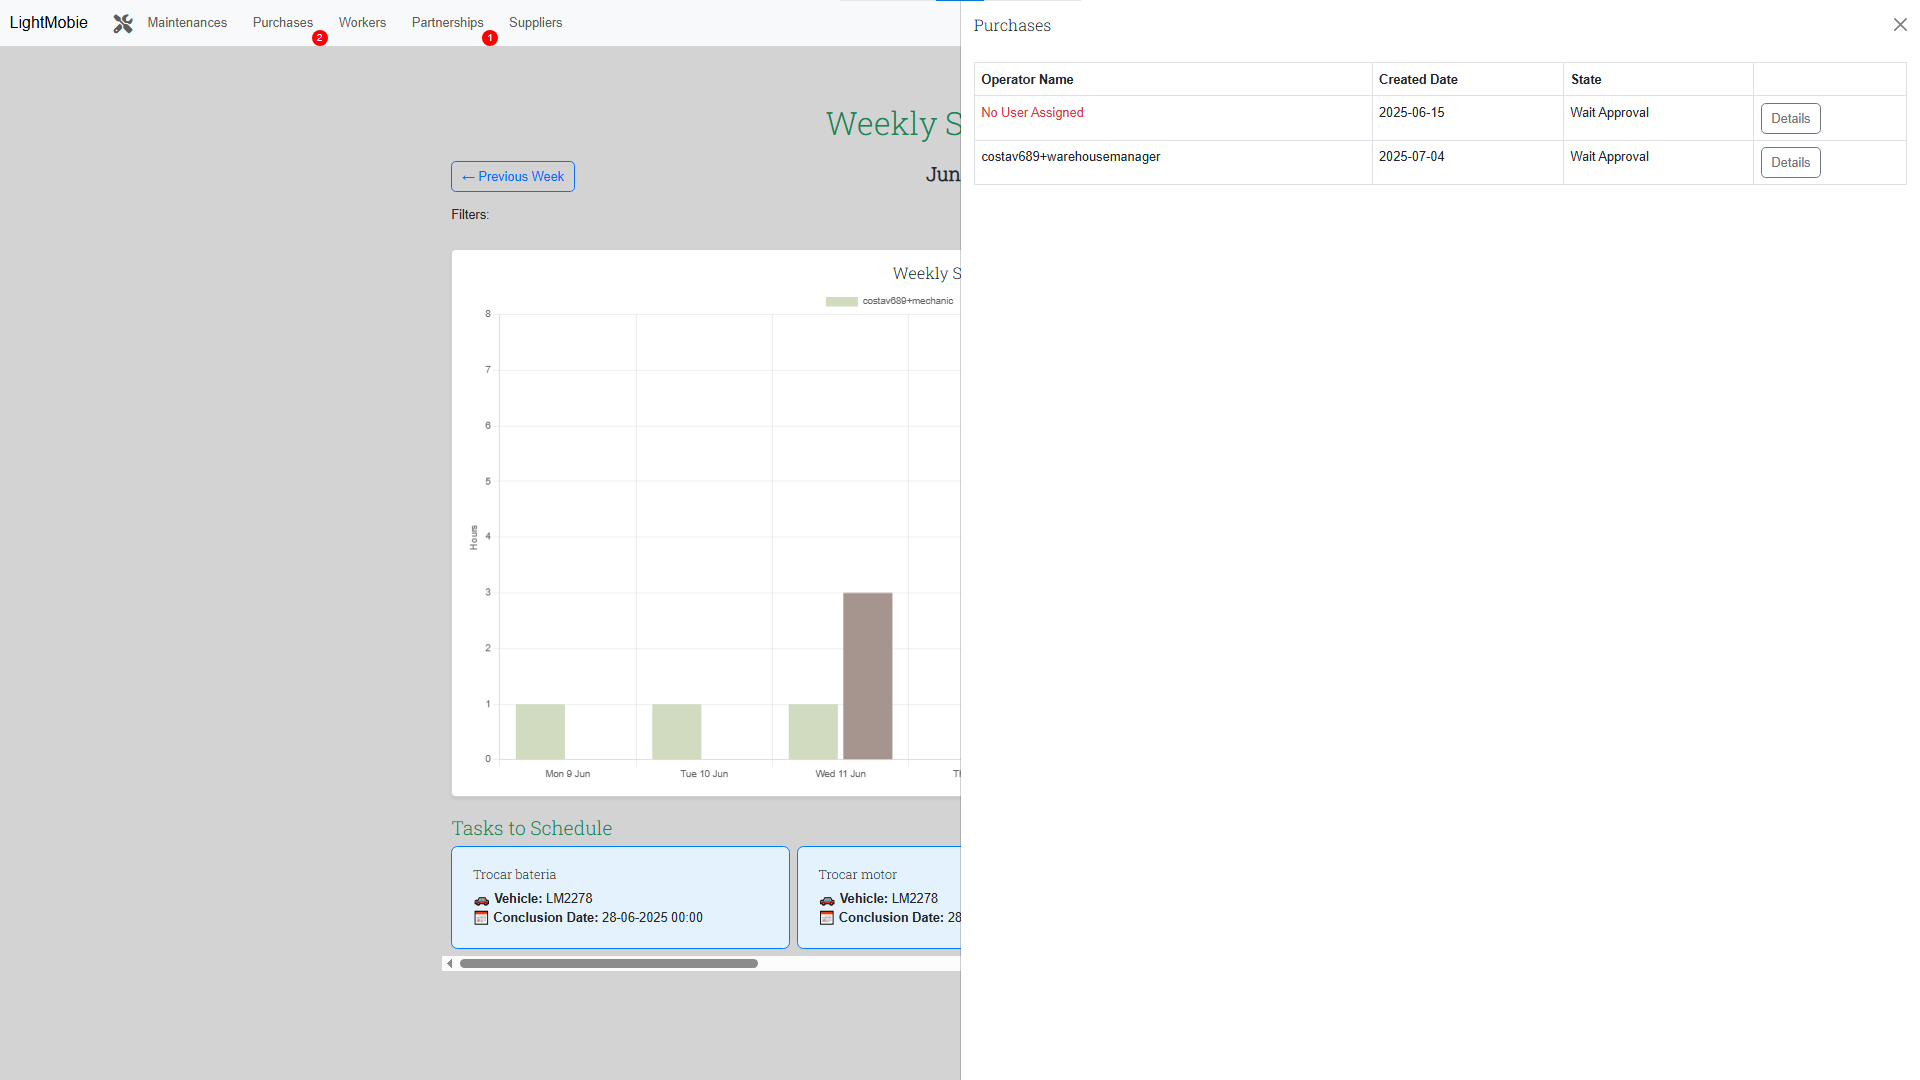
\includegraphics[width=\textwidth]{figs/Implementation/workshopmanager/purchaseList}
  \label{fig:workshopmanagerPurchaseList}
\end{figure}



Purchase management also extends the warehouse operator's functionality. Managers review purchase requests submitted by operators and either authorize or reject them (Use Case 4.2 – Authorize purchase). When authorizing, they may also add additional parts and assign the request to a specific operator (Figures~\ref{fig:workshopmanagerPurchaseList}-~\ref{fig:workshopmanagerPurchaseDetails}).


\begin{figure}[h]
  \caption{Worker list.}
  \centering
  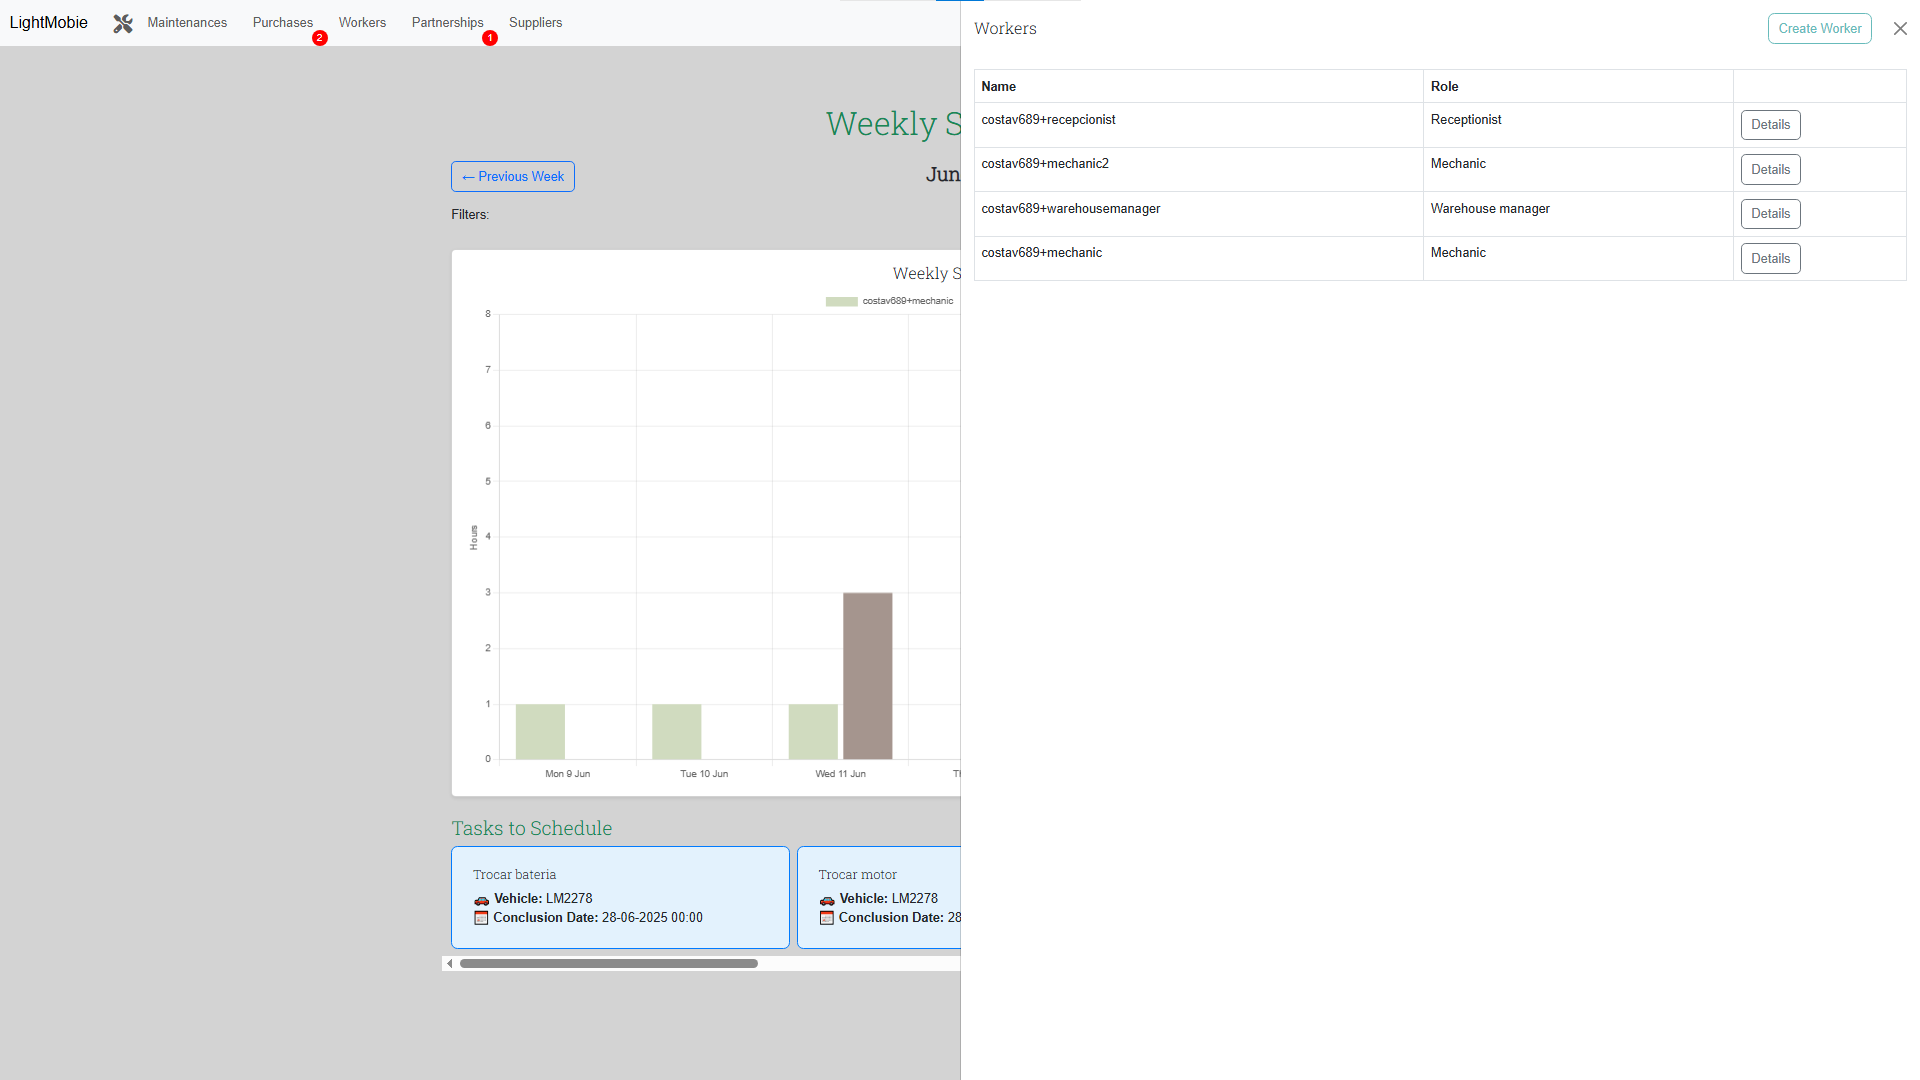
\includegraphics[width=\textwidth]{figs/Implementation/workshopmanager/workerList}
  \label{fig:workerList}
\end{figure}




The worker management module allows the manager to view dealership employees, edit their roles, and register new workers (Use Case 4.5 – Assign roles to employees). Each worker's details include personal information and role, with options to modify or remove them (Figures~\ref{fig:workerList}-~\ref{fig:workerCreate}).


\begin{figure}[h]
  \caption{Partnership list.}
  \centering
  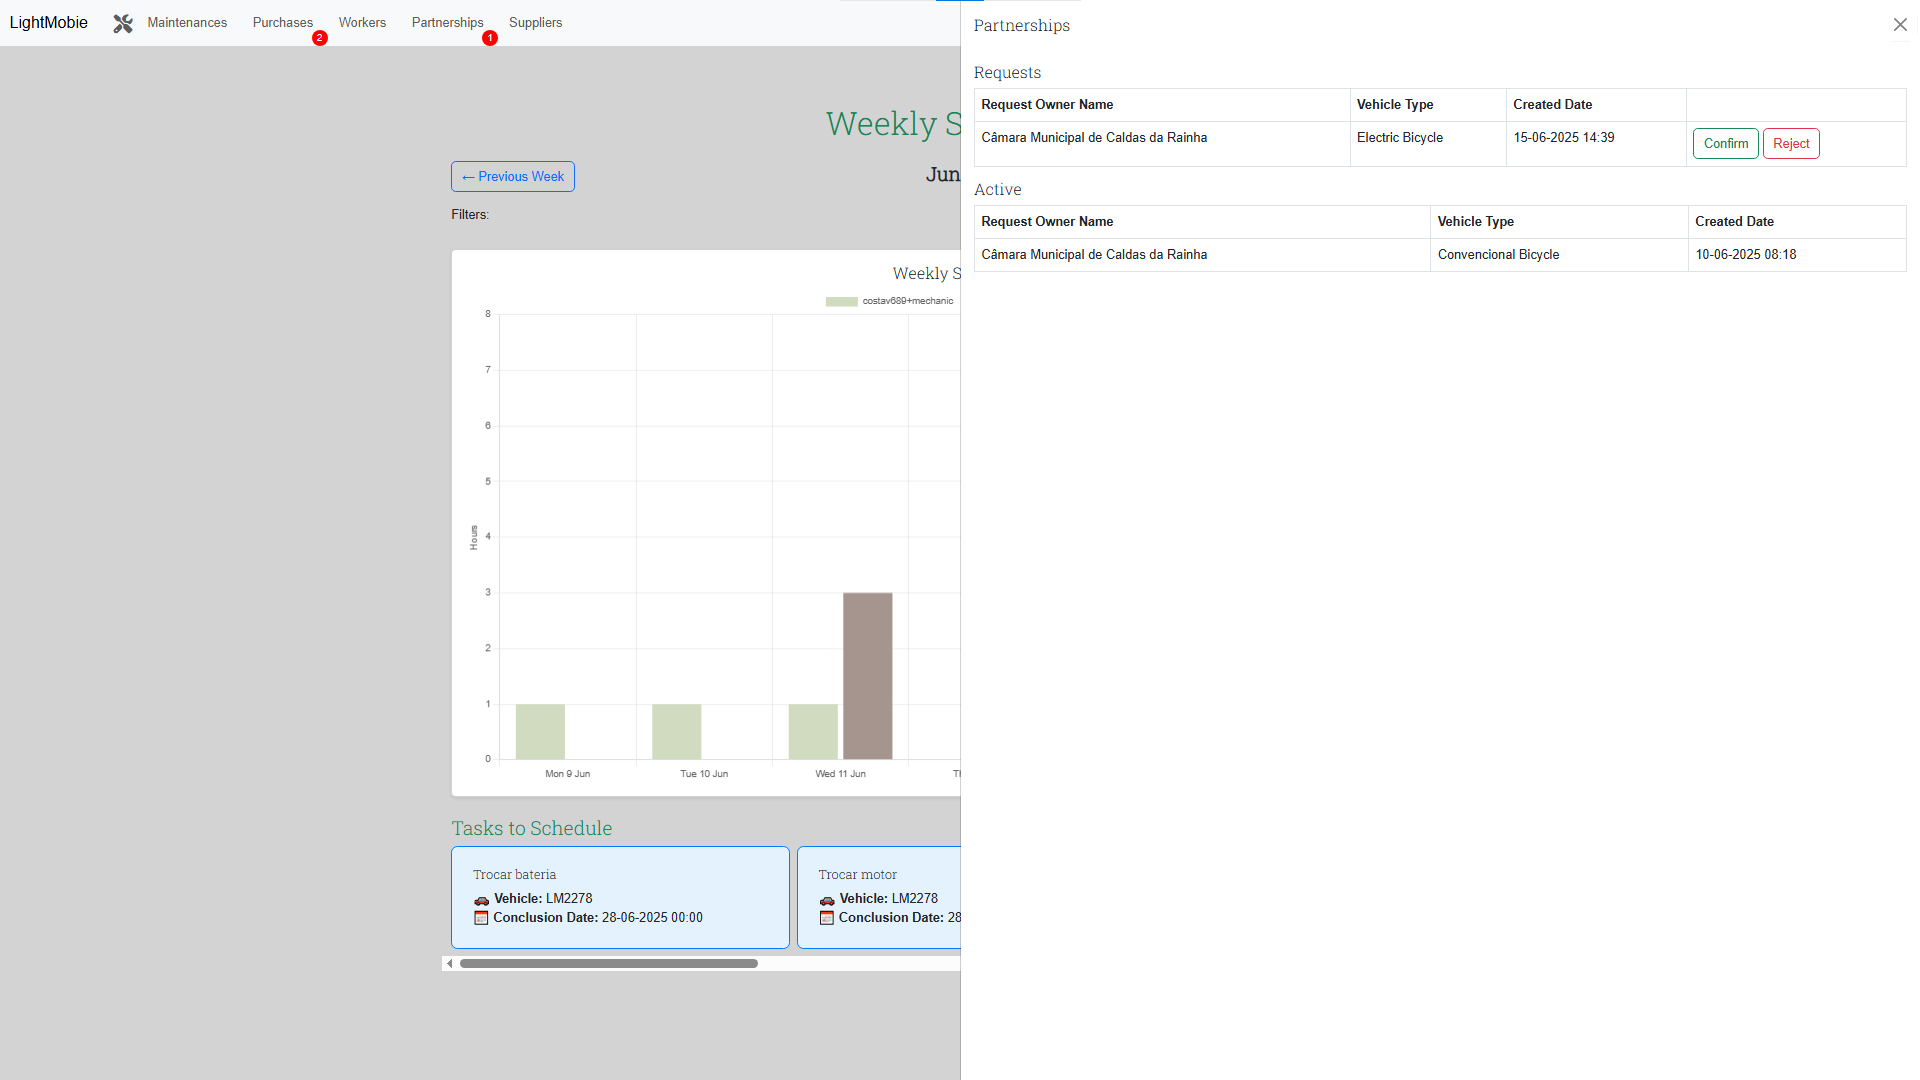
\includegraphics[width=\textwidth]{figs/Implementation/workshopmanager/partnershipList}
  \label{fig:partnershipList}
\end{figure}


Partnership requests are handled through a dedicated view. New partnership proposals from external entities list the entity name, vehicle types, and creation date, and can be either accepted or rejected (Use Case 4.8 – Accept/Reject partnership). Confirmed partners are displayed in a separate table (Figure~\ref{fig:partnershipList}).

Finally, supplier management is identical to the warehouse operator view, displaying supplier details, contact information, and contract terms for parts provided (Figures~\ref{fig:workshopmanagerSupplierList}-~\ref{fig:workshopmanagerupplierDetails}).



\subsection{Client view}

\begin{figure}[h]
  \caption{Client Home page when the vehicle evaluation is complete.}
  \centering
  
\includegraphics[width=\textwidth]{figs/Implementation/client/MaintenanceState2}
  \label{fig:MaintenanceState2}
\end{figure}


The client interface is designed for mobile use and focuses on tracking the status of a vehicle's maintenance. Its layout differs from the employee views by being streamlined and tailored to end-user needs.




\begin{figure}[h]
  \caption{Client Home page when the vehicle after the vehicle is delivered to the client.}
  \centering
  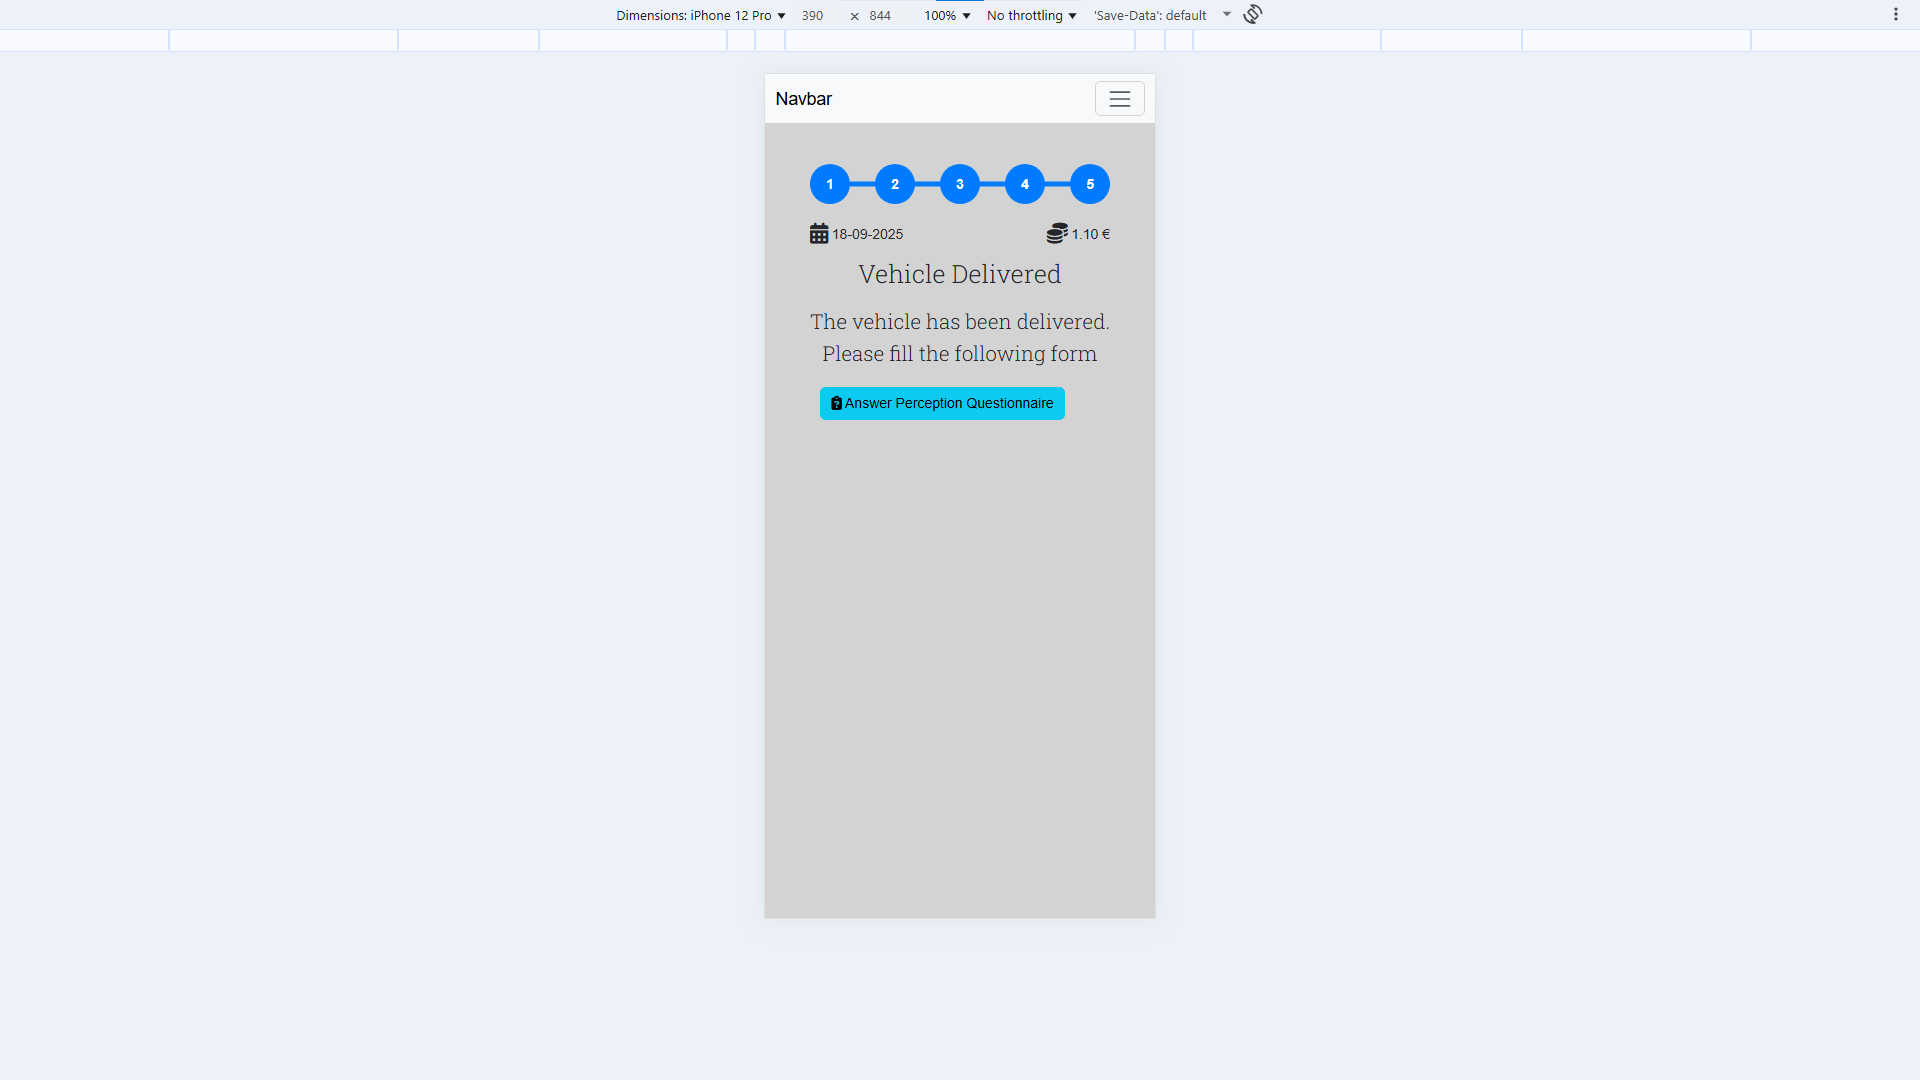
\includegraphics[width=\textwidth]{figs/Implementation/client/MaintenanceState5}
  \label{fig:MaintenanceState5}
\end{figure}



When a maintenance is scheduled with a dealership, the home page displays the upcoming evaluation date (Figure~\ref{fig:MaintenanceNoState}). Once the evaluation is complete, the client sees the list of proposed tasks, which must be confirmed before the maintenance proceeds (Figure~\ref{fig:MaintenanceState1}). After approval, the client can monitor task progress, following their completion status step by step (Figures~\ref{fig:MaintenanceState2}-~\ref{fig:MaintenanceState4}). During this phase, the client is invited to rate the expected service quality — the level of service they anticipate receiving during the maintenance — using the questionnaire in the second column of the Table~\ref{table:servqual_template} Figure~\ref{fig:ExpectationQuestionare}. When all tasks are finished, the application notifies the client that the vehicle is ready for pickup ( Figure~\ref{fig:MaintenanceState5}), and once the delivery is completed, the client can rate the perceived service quality, using the questionaire in the third column of the Table~\ref{table:servqual_template}, as seen in Figure~\ref{fig:PerceptionQuestionare}.

\begin{figure}[h]
  \caption{List of completed maintenances of the client.}
  \centering
  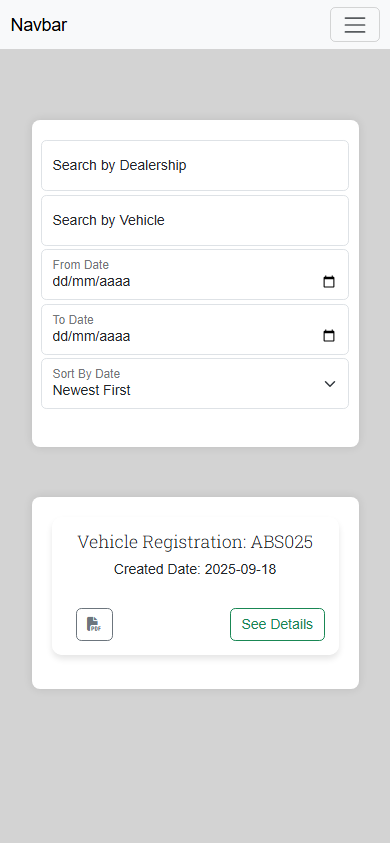
\includegraphics[width=\textwidth]{figs/Implementation/client/MaintenanceHistory}
  \label{fig:clientMaintenanceHistory}
\end{figure}


In addition to active maintenances, clients can review their full maintenance history (Use Case 5.5 – View maintenance history). The history view supports filtering by vehicle, dealership, or date (Figure~\ref{fig:clientMaintenanceHistory}). For each entry, clients may download a PDF report—identical to the one generated by the workshop manager—or open a detailed modal with information and task breakdowns (Figures~\ref{fig:MaintenanceDetailsInfo},~\ref{fig:MaintenanceDetailsTasks} and~\ref{fig:report}).



\subsection{Administrator view}


\begin{figure}[h]
  \caption{Parts type list.}
  \centering
  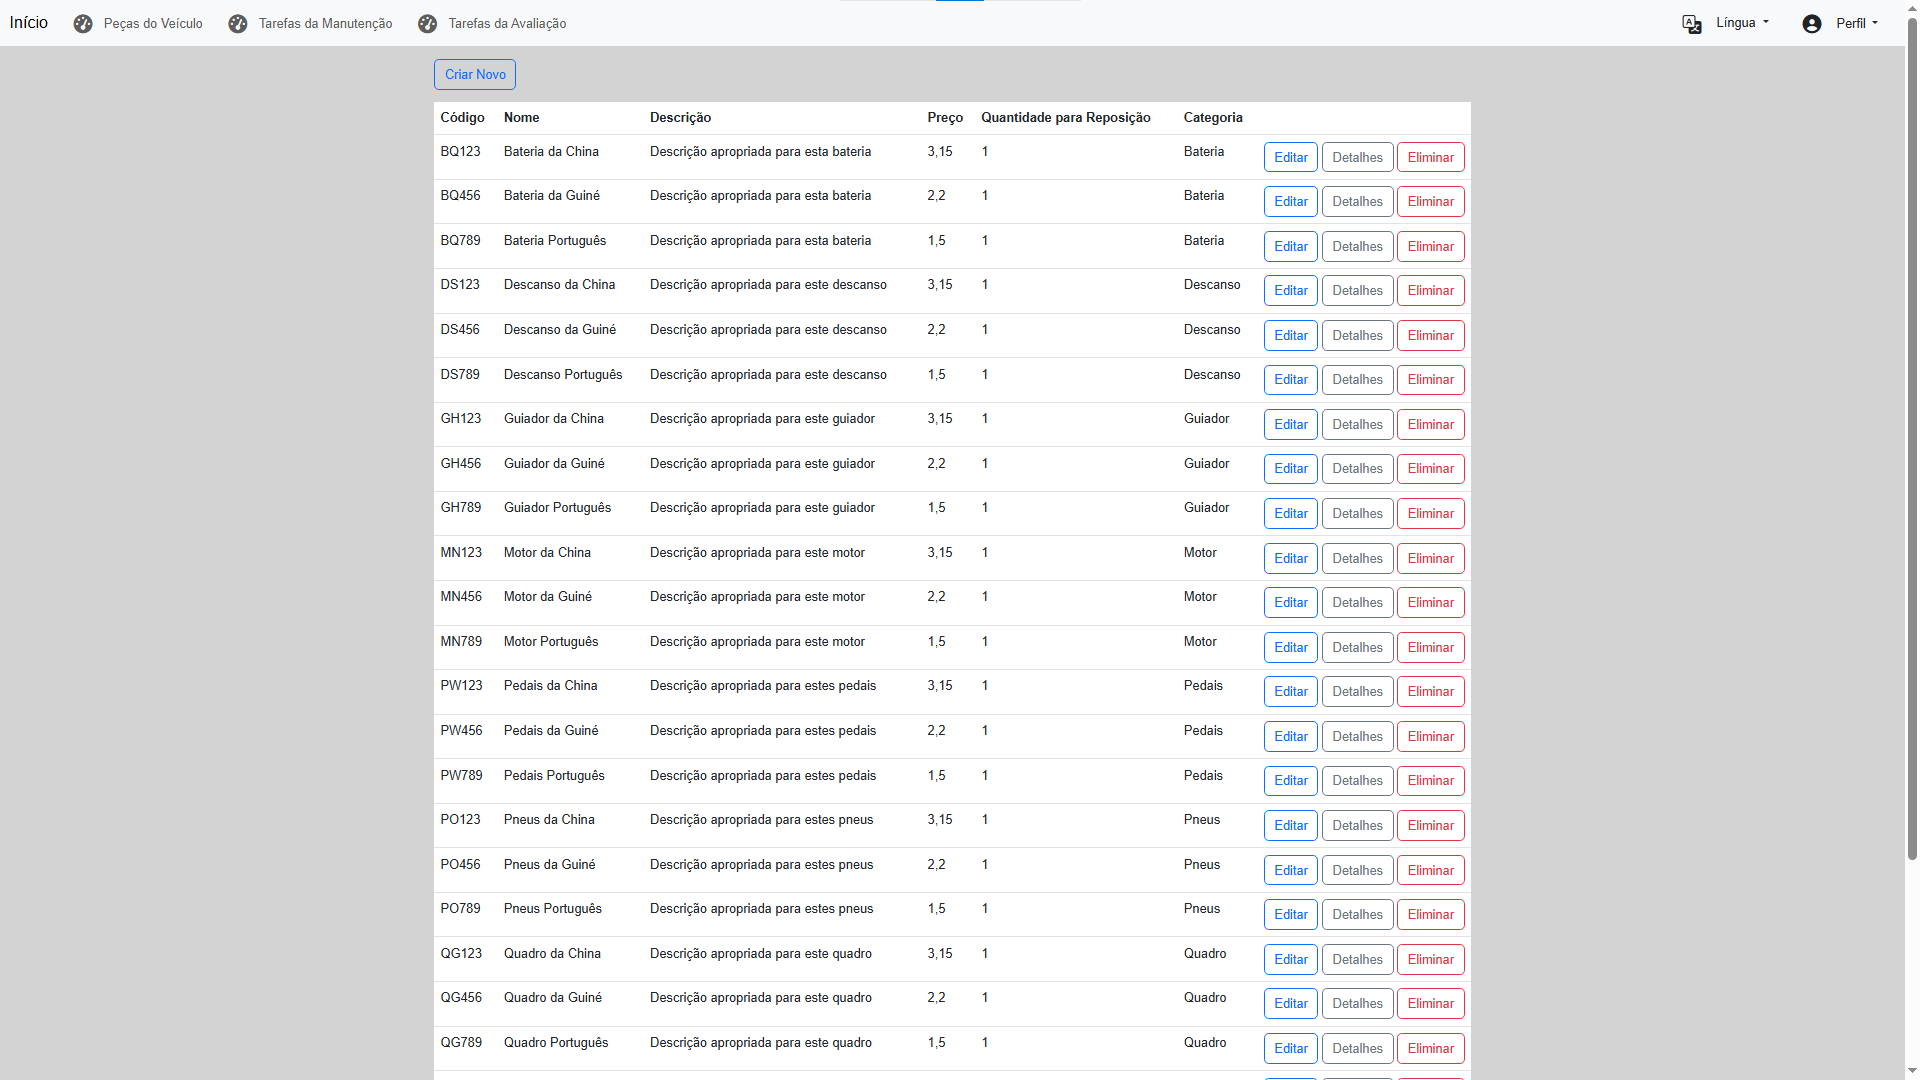
\includegraphics[width=\textwidth]{figs/Implementation/dealershipAdmin/partsIndex}
  \label{fig:partsIndex}
\end{figure}



The administrator interface is dedicated to configuring the system's core information, namely the catalog of parts, task types, and evaluation tasks. Upon logging in, the administrator is presented with a list of part types (Figure~\ref{fig:partsIndex}). From this view, parts can be created, edited, deleted, or inspected in detail (Figures~\ref{fig:partsDetails}-~\ref{fig:partsDelete}). Each operation follows the same interaction pattern: selecting an action in the table opens a form or details modal, ensuring consistency and efficiency.




The same layout is applied to managing task types (Figures~\ref{fig:taskIndex}-~\ref{fig:taskCreate}) and evaluation tasks (Figures~\ref{fig:evalIndex}-~\ref{fig:evalEdit}), maintaining uniformity across all system configuration sections. This design allows the administrator to quickly perform updates with minimal effort, ensuring that the dealership's catalog of parts and tasks remains accurate and up to date.


\subsection{Summary}

In summary, the implementation of the different application views demonstrates that the overall system requirements were successfully met. Each user role — receptionist, workshop manager, mechanic, warehouse operator, client, and administrator — was provided with a tailored interface designed to support their specific tasks. Although some views share similarities in layout and functionality, they each incorporate the particular features required to fulfill their responsibilities. 






